% -*- coding: iso-latin-1 -*-
%
% SUMMARY:
% USAGE:
%
% AUTHOR:       Christophe Prud'homme
% ORG:          Christophe Prud'homme
% E-MAIL:       prudhomm@zion
%
% ORIG-DATE:  7-Apr-04 at 16:48:32
% LAST-MOD:  7-Apr-04 at 23:07:19 by Christophe Prud'homme
%
% DESCRIPTION:
% DESCRIP-END.

\date{January 21 2008}

\begin{document}

% For every picture that defines or uses external nodes, you'll have
% to apply the 'remember picture' style. To avoid some typing, we'll
% apply the style to all pictures.
\tikzstyle{every picture}+=[remember picture]
\tikzstyle{na} = [baseline=-.5ex]

%By default all math in TikZ nodes are set in inline mode. Change this to
% displaystyle so that we don't get small fractions.
\everymath{\displaystyle}

\lecture[3]{Polynomial Approximation}{approx}
\subtitle{}

\begin{frame}
  \maketitle
\end{frame}

\begin{frame}
  \tableofcontents
\end{frame}

\begin{frame}{Introduction}
  We now describe the operations on the reference element $\Omst$
  \begin{itemize}
  \item Definition of $\Omst$
  \item Construction of  polynomials
  \item Evaluation of  polynomials
  \item Differentiation of polynomials
  \item Other operation: addition, substraction, integration, $\nabla
    \cdot$, $\nabla \times$, ...
  \end{itemize}
\end{frame}

\section{Geometry}
\label{sec:geometry}


\begin{frame}[containsverbatim]{Reference Convex ${K}$}
  \begin{columns}[c]
    \begin{column}{.4\textwidth}
      \begin{figure}[H]
        \centering
        %% \movie[externalviewer=kaffeine,label=diphase]{\pgfuseimage{tetra-2}}{}
        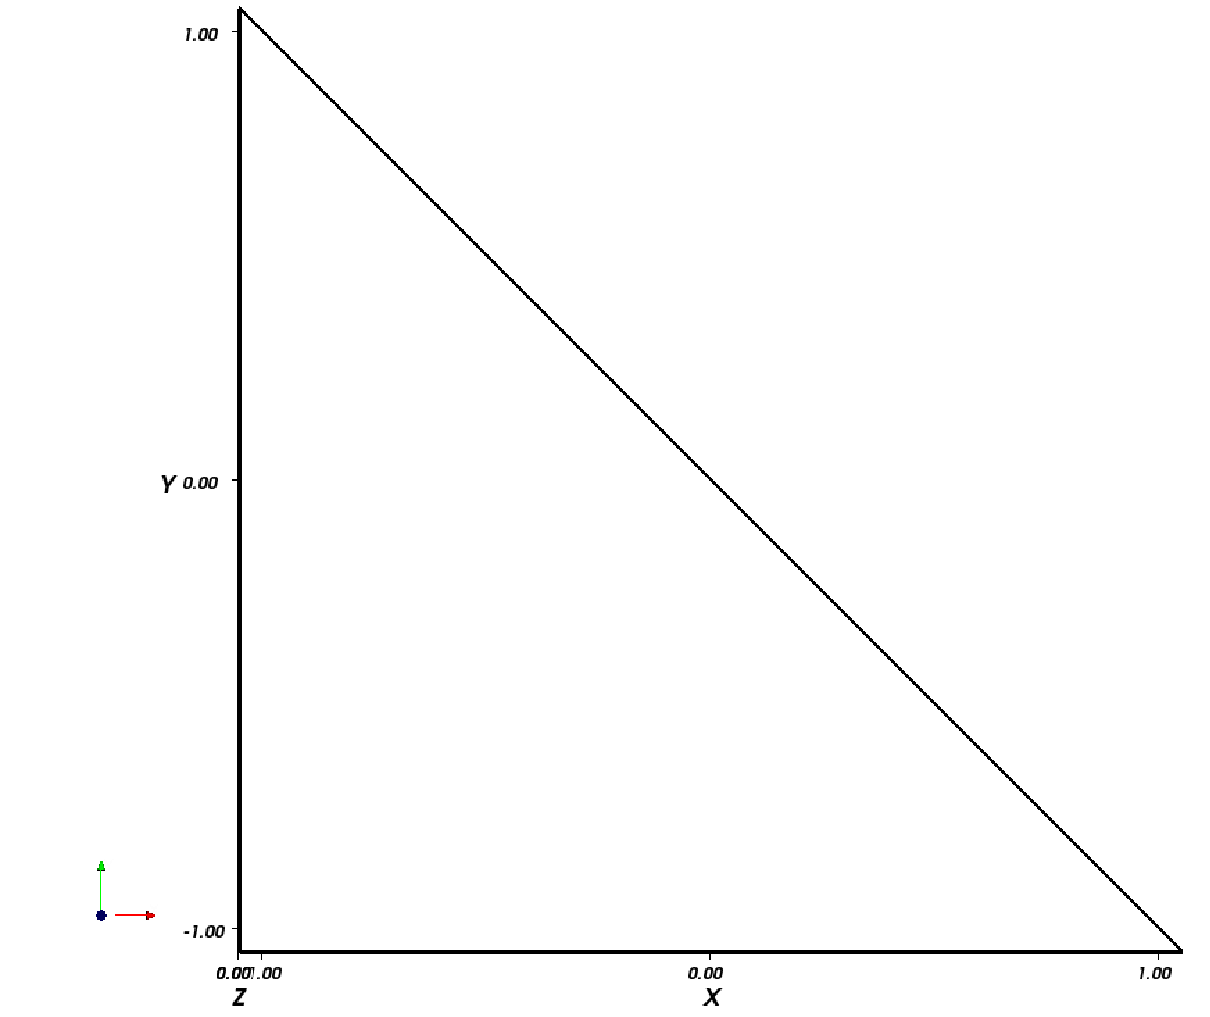
\includegraphics[width=\figwidth\textwidth]{../figures/triangle.pdf}\\
        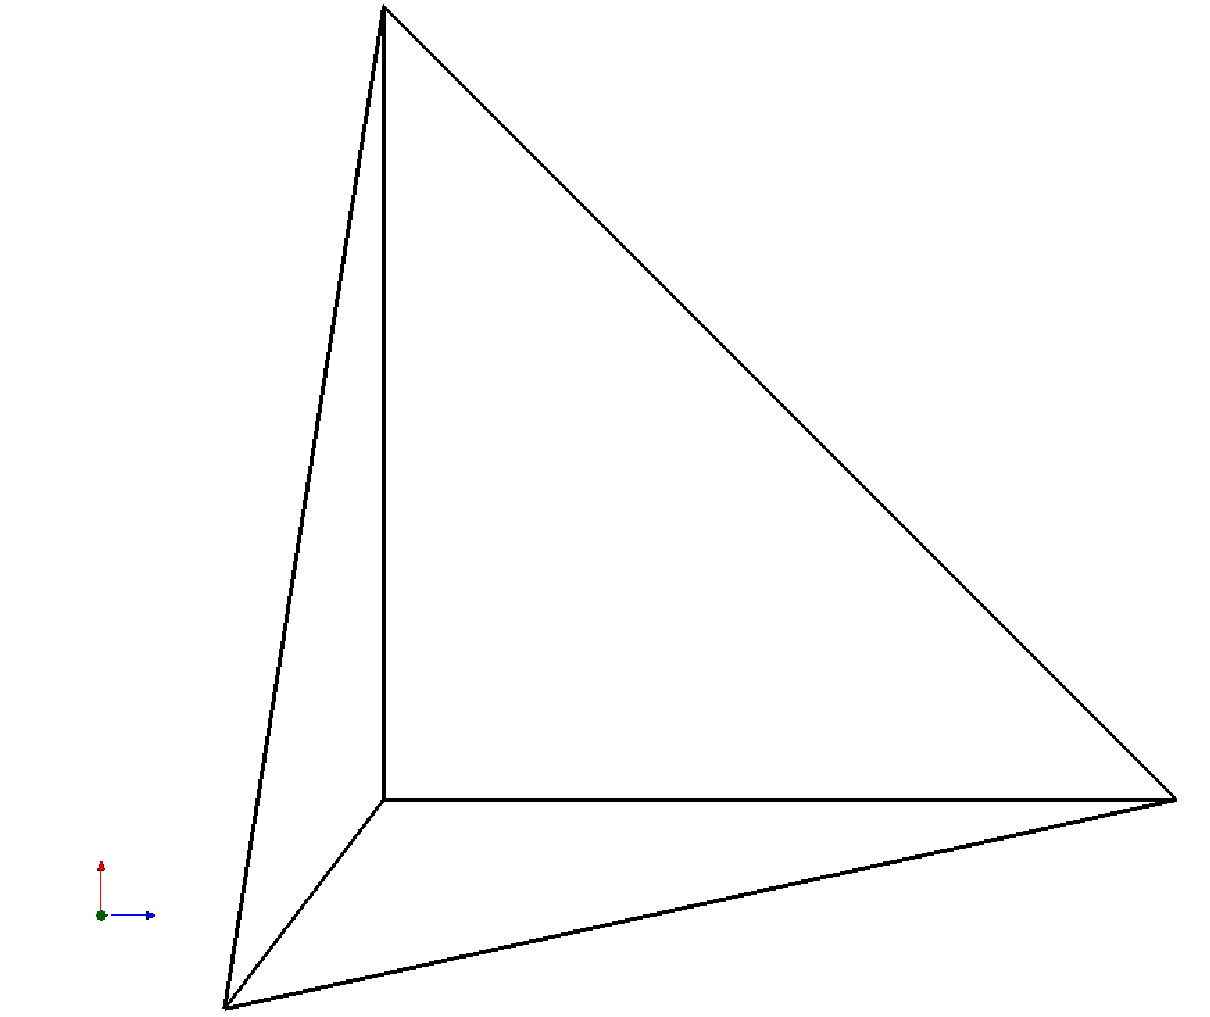
\includegraphics[width=\figwidth\textwidth]{../figures/tetra.pdf}
        %% \hyperlinkmovie[externalviewer=kaffeine]{diphase}{\beamergotobutton{Film}}
        \caption{Simplexe de R�f�rence en 2D/3D}
      \end{figure}
    \end{column}
    \begin{column}{.6\textwidth}
      \begin{block}{}
        \begin{itemize}
        \item Simplices, $d=1,2,3$
          \alert{collapsed coordinates}
        \item Simplex products
        \item Orientation
        \item Normals, Tangents
        \end{itemize}
      \end{block}
      \begin{alertblock}{Crucial}
        Decomposition of convexes into its sub-entities (volume,
        faces, edges, points) and in an ordered manner
      \end{alertblock}


% \begin{lstlisting}[]
% template<uint16_type Dim,
%          uint16_type Order = 1,
%          uint16_type RealDim = Dim,
%          typename T = double>
% class Simplex {
%  // Informations statiques
%  // orientation
%  // points
%  // points par entit�s g�om�triques
%  // normales/tangentes
%  // ...
% };
% \end{lstlisting}
    \end{column}
  \end{columns}
\end{frame}
\subsection{Interval}
\begin{frame}[containsverbatim]{The interval $[-1;1]$}
  An interval is composed of
  \begin{itemize}
  \item two vertices
  \item an edge connecting the two vertices
  \end{itemize}
  \begin{figure}[H]
    \centering
    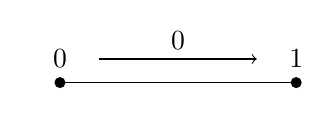
\begin{tikzpicture}[scale=2]
      \tikz {
        \fill (0,0) circle (2pt) node[above=2pt] {0};
        \draw (0,0)  to[line to] (3,0);
        \draw[->] (0.5,0.3)  to[line to] node[above] {0} (2.5,0.3) ;
        \fill (3,0) circle (2pt) node[above=2pt] {1};
      }
    \end{tikzpicture}
    \caption{Local and global numbering of the interval}
  \end{figure}
  Denote \lstinline!entity[0]! and \lstinline!entity[1]! the
  subentities sets for the vertices and edges respectively, we have
  \begin{itemize}
  \item \lstinline!entity[0] = {0,1}!
  \item \lstinline!entity[1] = {0}!
  \end{itemize}
\end{frame}

\subsection{Quadrilateral}
\begin{frame}[containsverbatim]{Quadrilateral}
  \begin{figure}[H]
    \centering
    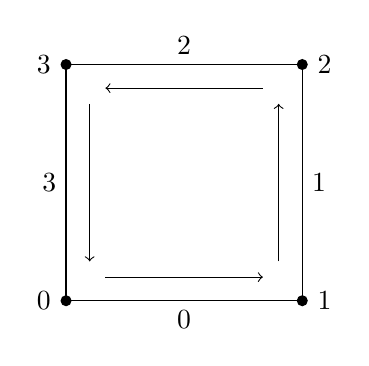
\begin{tikzpicture}[scale=1]
        \draw[->] (0.5,0.3)  to[line to]  (2.5,0.3) ;
        \draw[->] (2.7,0.5)  to[line to]  (2.7,2.5) ;
        \draw[->] (2.5,2.7)  to[line to]  (0.5,2.7) ;
        \draw[->] (0.3,2.5)  to[line to]  (0.3,0.5) ;


        \draw
        (0,0)  to[line to] node[below] {0} (3,0)
        (3,0)  to[line to] node[right] {1} (3,3)
        (3,3)  to[line to] node[above] {2} (0,3)
        (0,3)  to[line to] node[left]  {3} (0,0)
        ;
        \fill (0,0) circle (2pt) node[left=2pt] {0};
        \fill (3,0) circle (2pt) node[right=2pt] {1};
        \fill (3,3) circle (2pt) node[right=2pt] {2};
        \fill (0,3) circle (2pt) node[left=2pt] {3};
    \end{tikzpicture}

    \caption{Local numbering and orientation  for vertices and edges of the quadrilateral}
    \label{fig:2}
  \end{figure}
  We shall denote
  \begin{equation}
    \label{eq:2}
    \mathcal{Q}^2 = \{ (x_1, x_2) \in \setR{2} | -1 < x_1, x_2 < 1 \}
  \end{equation}
  We have for the quadrangle
  \begin{itemize}
  \item \lstinline!entity[0] = {0,1,2,3}!
  \item \lstinline!entity[1] = {0,1,2,3}!
  \item \lstinline!entity[2] = {0}!
  \end{itemize}
\end{frame}

\subsection{Triangle}
\begin{frame}[containsverbatim]{Triangles}
  \begin{figure}[H]
    \centering
    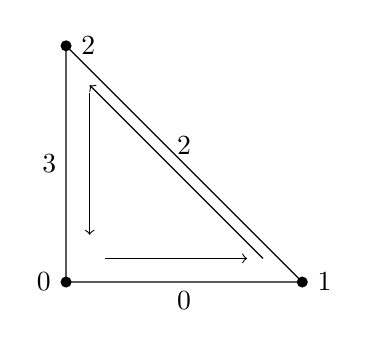
\begin{tikzpicture}[scale=1]
      \draw[->] (0.5,0.3)  to[line to]  (2.3,0.3) ;
      \draw[->] (2.5,0.3)  to[line to]  (0.3,2.5) ;
      \draw[->] (0.3,2.4)  to[line to]  (0.3,0.6) ;


      \draw
      (0,0)  to[line to] node[below] {0} (3,0)
      (3,0)  to[line to] node[above] {2} (0,3)
      (0,3)  to[line to] node[left]  {3} (0,0)
      ;
      \fill (0,0) circle (2pt) node[left=2pt] {0};
      \fill (3,0) circle (2pt) node[right=2pt] {1};
      \fill (0,3) circle (2pt) node[right=2pt] {2};
    \end{tikzpicture}

    \caption{Local numbering and orientation  for vertices and edges of the triangles}
    \label{fig:2}
  \end{figure}
  We shall denote
  \begin{equation}
    \label{eq:1}
    \mathcal{T}^2 = \{ (x_1, x_2) \in \setR{2} | -1 < x_1, x_2 < 1, x_1 + x_2 < 0 \}
  \end{equation}
  We have for the triangle
  \begin{itemize}
  \item \lstinline!entity[0] = {0,1,2}!
  \item \lstinline!entity[1] = {0,1,2}!
  \item \lstinline!entity[2] = {0}!
  \end{itemize}
\end{frame}

\subsection[Tet. and Hex.]{Tetrahedron and hexahedron}
\begin{frame}{Tetrahedron and hexahedron}
  We do a similar construction for the tetrahedron and hexahedron, i.e
  decompsoing it into vertices, edges, faces and volumes

  We shall denote
  \begin{equation}
    \label{eq:3}
    \mathcal{T}^3 = \{ (x_1, x_2, x_3) \in \setR{3} | -1 < x_1, x_2, x_3 < 1, x_1 + x_2 + x_3 < 0 \}
  \end{equation}
  and
  \begin{equation}
    \label{eq:4}
    \mathcal{Q}^3 = \{ (x_1, x_2, x_3) \in \setR{4} | -1 < x_1, x_2, x_3 < 1 \}
  \end{equation}
\end{frame}

\begin{frame}[containsverbatim]{C++}
\begin{lstlisting}
 template<uint16_type Dim,
          uint16_type RealDim = Dim>
 class Simplex {
  // static Informations
  // orientation
  // normales/tangentes
  // decomposition in subentities
  // routine to manipulate the subentities
 };
\end{lstlisting}

\end{frame}
\section{Polynomials Bases}
\label{sec:polynomials-bases}

\subsection[Space]{Polynomial Spaces}
\begin{frame}{Polynomial Spaces}
  Denote
  \begin{equation}
    \label{eq:5}
    \PS{N}(\GT{d}) = \{ p | \text{degree} \leq N \}
  \end{equation}
  and
  \begin{equation}
    \label{eq:6}
    \QS{N}(\GQ{d}) = \{ p | \text{degree} \leq N \text{ in each variable} \}
  \end{equation}
\end{frame}

\subsection[Jacobi]{Jacobi Polynomials}
\begin{frame}{Jacobi Polynomials}

  The Jacobi polynomials $P_k^{(\alpha,\beta)}$ of indices
  $\alpha,\beta > -1$ and degree $k \geq 0$ are a family of orthogonal
  polynomials on $(-1,1)$ w.r.t the inner product:
  \begin{equation}
    \label{eq:7}
    (u,v)_{(\alpha,\beta)} = \int_{-1}^1 \ u(x)\ v(x)\ (1-x)^\alpha\ (1+x)^\beta\ dx
  \end{equation}

  The polynomials can be calculated using the recurrence formulas [see Sherwin-Karnyadakis].

  \begin{block}{Remark}
    We are going to use the Jacobi polynomials using specific values
    of $\alpha$ and $\beta$. Note also that the \alert{roots} of these
    polynomials are crucial in the construction of quadrature formulas
    (we come back later to them)
  \end{block}
\end{frame}

\begin{frame}{Recurrence relations for evaluation}
  \begin{equation*}
    \label{eq:15}
  \begin{aligned}
    P_0^{\alpha,\beta}( x ) &= 1,\\
    P_1^{\alpha,\beta}( x ) &= \frac{1}{2}\Big[ \alpha -\beta +(\alpha+\beta+2)x \Big],\\
    a^1_n P_{n+1}^{\alpha,\beta}( x ) &= (a^2_n +a^3_n x) P_{n}^{\alpha,\beta}( x ) - a^4_n P_{n-1}^{\alpha,\beta}( x )\\
    a^1_n & = 2(n+1)(n+\alpha+\beta+1)(2n+\alpha + \beta)\\
    a^2_n & = (2n+\alpha+\beta+1)(\alpha^2 - \beta^2)\\
    a^3_n & = (2n+\alpha+\beta)(2n+\alpha + \beta+1)(2n+\alpha + \beta+2)\\
    a^4_n & = 2(n+\alpha)(n+\beta)(2n+\alpha + \beta+2)
  \end{aligned}

  \end{equation*}

  Some special values

  \begin{equation*}
    \begin{aligned}
      P_{n}^{\alpha,\beta}( 1 ) & =
      \begin{pmatrix}
        n+\alpha\\
        n
      \end{pmatrix} =
      \frac{(n+\alpha)!}{\alpha!n!}\\
      P_{n}^{\alpha,\beta}( -x ) & = (-1)^n P_{n}^{\alpha,\beta}( x )
    \end{aligned}

  \end{equation*}
\end{frame}
\begin{frame}{Recurrence relations for diffentiation}
  \begin{equation*}
    \label{eq:15}
  \begin{aligned}
    b^1_n \frac{d}{dx} P_n^{\alpha,\beta}( x ) &= b^2_n P_{n}^{\alpha,\beta}( x ) + b^3_n P_{n-1}^{\alpha,\beta}( x )\\
    b^1_n & = (2n+\alpha + \beta)(1-x^2)\\
    b^2_n & = n\Big[ \alpha -\beta -(\alpha+\beta+2n)x \Big]\\
    b^3_n & = 2(n+\alpha)(n+\beta)
  \end{aligned}
  \end{equation*}

\end{frame}



\subsection[Moment]{Moment basis}
\label{sec:moment-basis}

\begin{frame}{Moment basis}
  The moment basis is the canonical basis for the spaces $\PS{N}(\GT{d})$ or $\QS{N}(\GQ{d})$
  \begin{equation}
    \label{eq:8}
    \PS{N}(\GT{d}) =
    \begin{cases}
      x^i, & i \leq N,\\
      x^i y^j & i+j \leq N, \\
      x^i y^j  z^k & i+j+k \leq N,
    \end{cases}
  \end{equation}
  and
  \begin{equation}
    \label{eq:9}
    \QS{N}(\GQ{d}) =
    \begin{cases}
      x^i, & i \leq N,\\
      x^i y^j & i,j \leq N, \\
      x^i y^j z^k & i,j,k \leq N,
      \end{cases}
  \end{equation}

  \begin{block}{Remarks}
    \begin{description}
    \item[GOOD] Easy to construct and compute
    \item[GOOD] Easy Integration, differentiation
    \item[GOOD] Hierarchical basis
    \item[BAD] Very bad Vandermonde matrix conditioning as polynomial degree increases
    \item[BAD] Very bad mass matrix conditioning as polynomial degree increases
    \end{description}
  \end{block}
\end{frame}

\subsection{Legendre}
\begin{frame}{Tensorized Legendre Basis}
  Take $\alpha = \beta = 0$ in the Jacobi polynomials definition. we
  denote $L_k$ the $k$-th Legendre polynomial. $(L_k)_{k=1,...,N^d}$
  form a basis of $\QS{N}(\GQ{d})$.

  \begin{figure}[H]
    \centering
    \subfigure[Legendre]{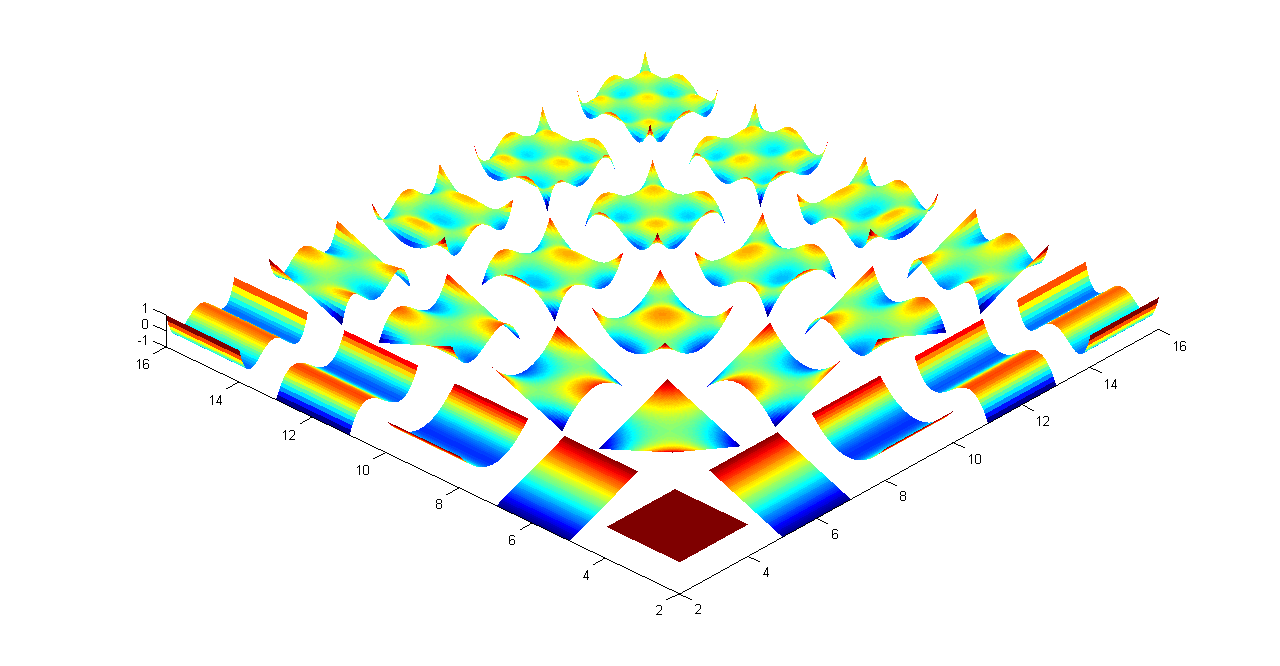
\includegraphics[width=\figwidth\textwidth]{../figures/Jacobi_2D}}
    \caption{Legendre polynomials in 2D and basis of $\QS{4}(\GQ{2})$. }
    \label{fig:3}
  \end{figure}
\end{frame}

\begin{frame}{Construction}
  \begin{itemize}
  \item The extension of 1D basis to quadrilaterals or hexahedra is done by \alert{tensorisation}.
  \item Consider $d$ 1D basis $\{ \varphi^{(l)}_{k_l}\}_{l=1}^d$ defined in $\GQ{1}$, the family $\{\phi_{\mathbf{k}}(\mathbf{x})\}_k$  given by
    \begin{equation}
      \label{eq:10}
      \phi_{\mathbf{k}}(\mathbf{x}) = \Pi_{l=1}^d\ \varphi^{(l)}_{k_l}( x_l ),\quad \mathbf{k} = (k_1,...,k_d), \mathbf{x}=(x_1,...,x_d)
    \end{equation}
    is a basis of $\QS{N}(\GQ{d})$
  \end{itemize}
  \begin{block}{Remark}
    \begin{description}
    \item[MODERATE BAD] moderate construction complexity
    \item[GOOD] $L_2$ orthogonal (normal) basis
    \item[GOOD] Hierarchical basis
    \item[GOOD] good (constant) mass matrix conditioning as polynomial degree increases
    \end{description}
  \end{block}
\end{frame}


\subsection{Dubiner}
\begin{frame}{Dubiner Basis}

  The Dubiner basis is an orthogonal modal basis on the simplices
  $\GT{d}$. Their construction derives from Legendre by collapsing
  vertices (i.e. introducing a collaped coordinate system)

  \begin{eqnarray}
    \label{eq:11}
    m: \GT{2} \mapsto \GQ{2},& (x_1,x_2) \rightarrow (\xi_1, \xi_2) &= \Big( 2\frac{1+x_1}{1-x_2}-1, x_2 \Big)\\
    m^{-1}: \GQ{2} \mapsto \GT{2},& (\xi_1,\xi_2) \rightarrow (x_1, x_2) &= \Big( \frac{1}{2}(1+\xi_1)(1-\xi_2)-1,\xi_2\Big)
  \end{eqnarray}

  We define now on the interval the following \alert{principal} functions
  \begin{equation}
    \label{eq:12}
    \left.
      \begin{array}{l}
	\psi_{p}(\xi) = P_{p}^{(0,0)}(\xi) \\
	\psi_{pq}(\xi) = \Big(\frac{1-\xi}{2}\Big)^{p}P_{q}^{(2p+1,0)}(\xi) \\
	\psi_{pqr}(\xi) = \Big(\frac{1-\xi}{2}\Big)^{p+q}P_{r}^{(2p+2q+2,0)}(\xi)
      \end{array}
    \right.
  \end{equation}
  The Dubiner basis reads in 2D and 3D as follows:
  \begin{equation}
    \label{eq:14}
    \begin{array}[c]{rl}
    \phi_{k_1,k_2}(x_1,x_2) &= \psi_{k_1}(\xi_1)	\psi_{k_1,k_2}(\xi_2)\\
    \phi_{k_1,k_2,k_3}(x_1,x_2,x_3) &= \psi_{k_1}(\xi_1)	\psi_{k_1,k_2}(\xi_2) \psi_{k_1,k_2,k_3}(\xi_3)
  \end{array}
  \end{equation}
  The cardinality is $(N+1)(N+2)/2$ in 2D and $(N+1)(N+2)(N+3)/6$.
\end{frame}
\begin{frame}{Dubiner basis in 2D}
  \begin{figure}[H]
    \centering
    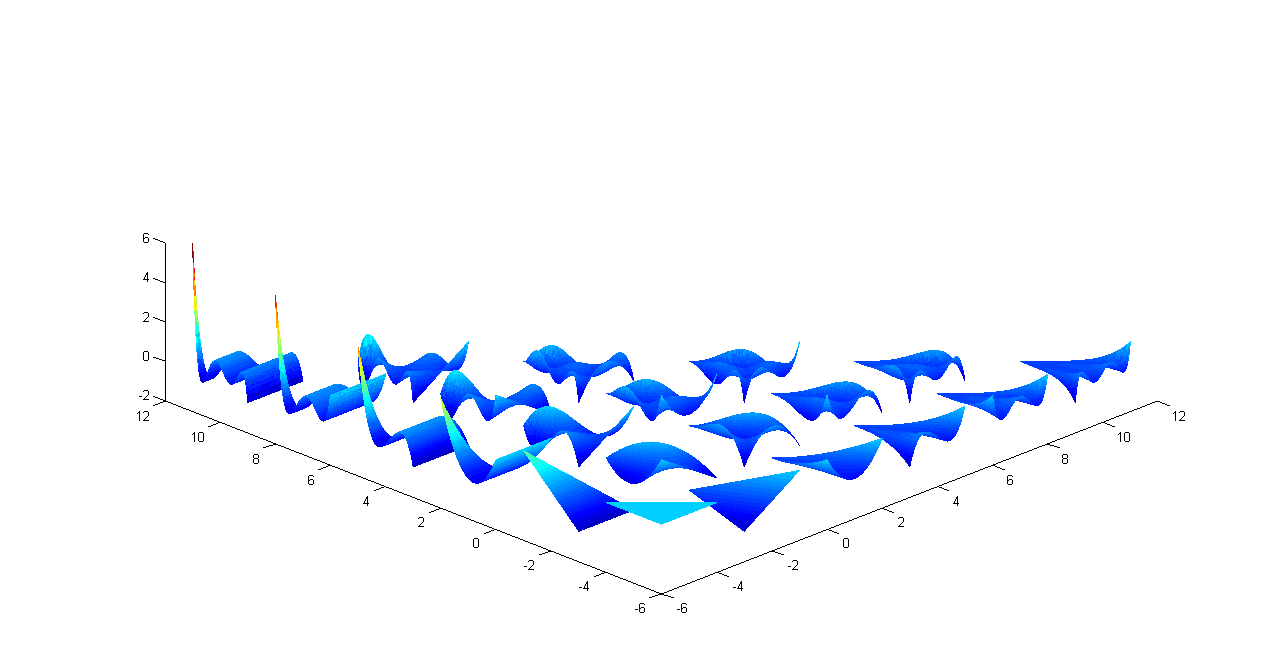
\includegraphics[width=\figwidth\textwidth]{../figures/Dubiner_5}
    \caption{Dubiner polynomials in 2D and basis of $\PS{5}(\GQ{2})$. }
    \label{fig:3}
  \end{figure}
\end{frame}

\section[FEM]{Finite element method}
\label{sec:finite-elem-meth}


\begin{frame}{Objective}

  \begin{block}{Finite/Spectral-hp element in 1/2/3D}
    \centerline{Construct {\LARGE$ (\ {K},\ {\mathbb{P}},\ {\Sigma}\ )$}}

    \begin{itemize}
    \item ${K}$ Reference convex
    \item ${\mathbb{P}}$ polynomial space
    \item ${\Sigma}$ dual space (degrees of freedom)
    \end{itemize}
    \hfill (Ciarlet, Ern \& Guermond, R.C. Kirby(Fenics/FIAT),
    Sherwin/Karniadakis, Quarteroni et al.)
  \end{block}

  % \begin{alertblock}{Standards}
  %   \begin{itemize}
  %   \item Le formalisme math�matique ci-dessus est rarement
  %     pr�sent/explicite dans les codes
  %   \item Souvent les �l�ments sont cod�s explicitement
  %     \begin{itemize}
  %     \item extension ordre �lev� difficile
  %     \item certains �l�ments rarement/jamais utilis�s car trop
  %       complexes ou pas de forme explicite
  %     \end{itemize}
  %   \end{itemize}
  % \end{alertblock}

  \note{\begin{itemize}
    \item G�om�trie �l�mentaire sur des convexes $\subset \mathbb{R}^d$
      (simplexes et produits de simplexes)
    \item Construction de familles de points dans les convexes de
      r�f�rences
    \item Construction de familles de polyn�mes sur les convexes de
      r�f�rences
    \item Construction d'un langage pour les formulations
      variationnelles
    \end{itemize}}
\end{frame}

\subsection{Point sets}

\begin{frame}{Points Sets in a Convex}

\begin{columns}
  \begin{column}[c]{.4\textwidth}
    \begin{figure}[H]
      \centering
      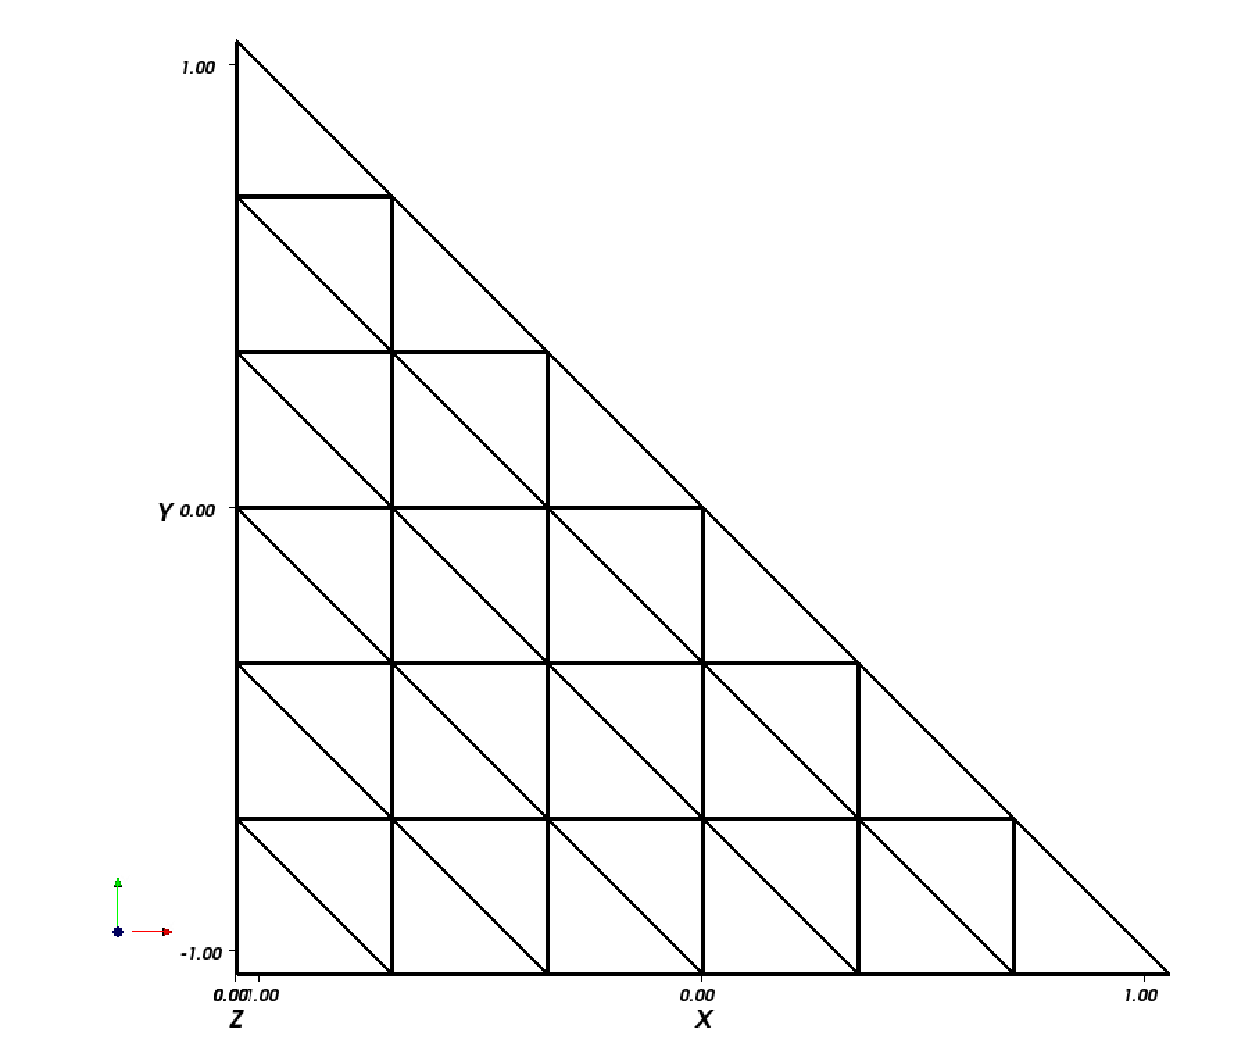
\includegraphics[width=0.7\textwidth]{../figures/triangle-equirepartis}\\
      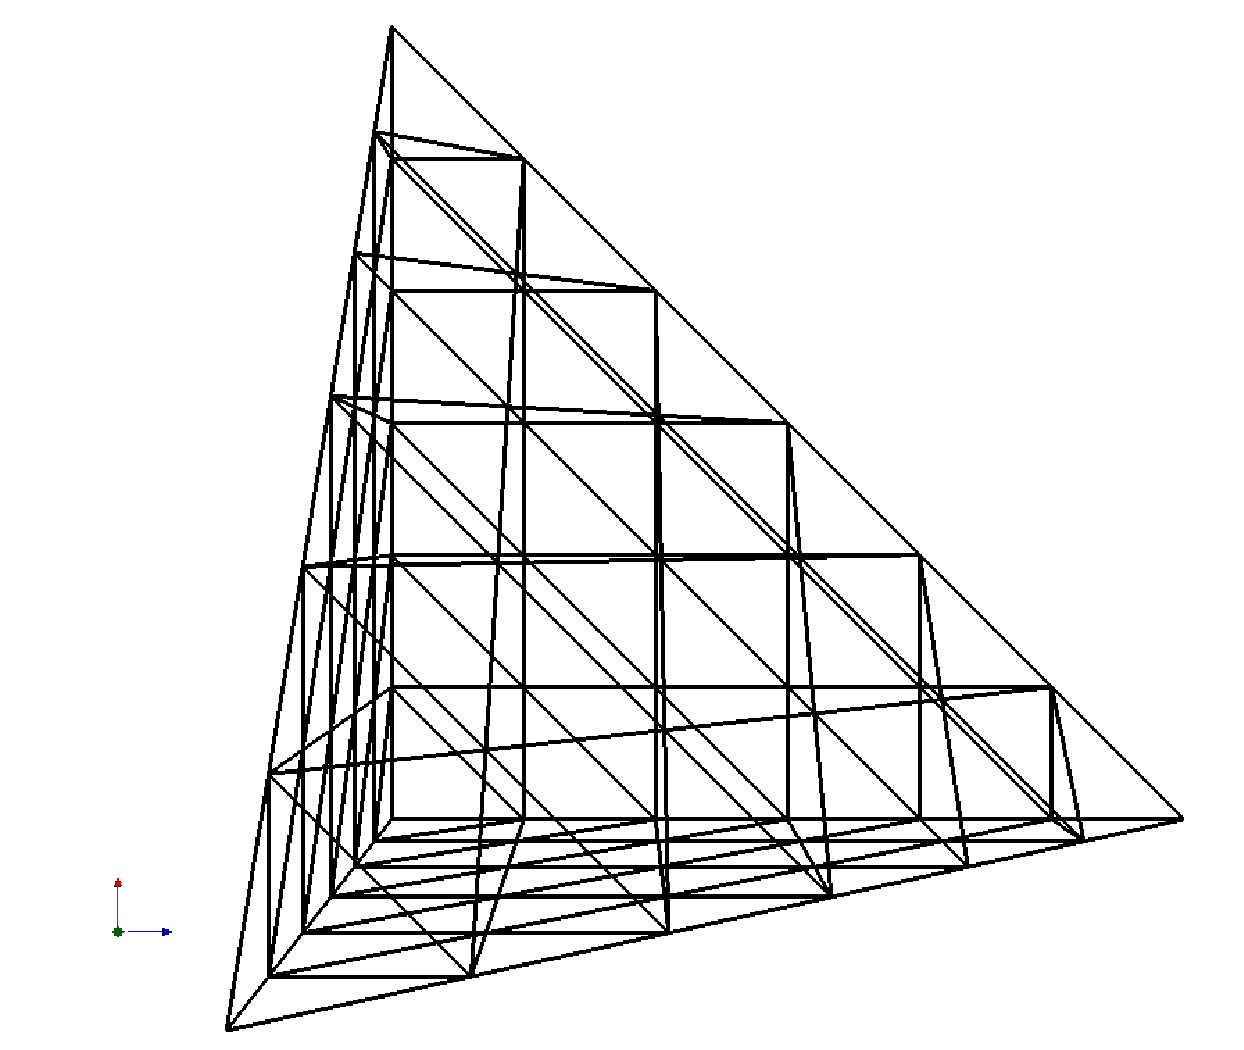
\includegraphics[width=0.7\textwidth]{../figures/tetra-equirepartis}
      \caption{\scriptsize Equi-distributed points in 2D/3D}
    \end{figure}
  \end{column}
  \begin{column}[c]{.6\textwidth}
    \begin{block}{Point Set $\{x_i\}_{i=1,N_p} \in K \subset \mathbb{R}^d$}
    \begin{itemize}
    \item Equi-distributed points
    \item Quadrature points, combination of
      \begin{itemize}
      \item Legendre
      \item Lobatto
      \item Radau
      \end{itemize}
    \item Interpolation points
      \begin{itemize}
      \item Fekete
      \item WarpBlend (explicit)
      \end{itemize}
    \item Algebraic representation: column oriented matrix ($d \times N_p$)
    \end{itemize}
    \hfill (Karniadakis \& Sherwin, Heasthaven, Warburton, Roth)
  \end{block}
  \end{column}
\end{columns}
\end{frame}
\begin{frame}{Construction}
  It is \alert{crucial} that all point sets are constructed with
  respect to the subentities of the reference domain for the DOF table
  construction ($C^0$ expansion or integration of faces)

  So if a point set of $N$ points in $\setR{d}$ is represented by a $d
  \times N $ matrix then
  \begin{itemize}
  \item first the points associated with vertices (wrt vertex ordering)
  \item then the points associated with the edges (wrt to edge ordering)
  \item  then the points associated with the faces (wrt to face ordering)
  \item  then the points associated with the volume
  \end{itemize}
\end{frame}
\begin{frame}[containsverbatim]{C++}
  \begin{lstlisting}
#include <boost/numeric/ublas/matrix.hpp>
template<class Convex,typename T>
class PointSet
{
  public:
  Convex convex() const { return M_convex; }
  uint16_type nPoints();
  // matrix column oriented
  // rows (coord.)
  // cols (points)
  points_type points() { return M_pts; }

  protected:
  ublas::matrix<T,row_major> M_pts;
};
template<class Convex,typename T>
class PointSetEquidistributed:
public PointSet
{
  // construction of the point set
};
  \end{lstlisting}
\end{frame}

\subsection{Polynomial set}
\begin{frame}[label=pset]{Polynomials and Polynomial Sets}

  \begin{block}{}
    Express the polynomials of $\Pk$ in the Dubiner basis $\{\phi_i\}_{i=1,\mathrm{dim} \Pk}$
    $$p=\sum_i (p, \phi_i)_K \phi_i,\quad p \in \Pk$$
    \begin{itemize}
    \item \alert{$L_2$ orthonormality}:
      \begin{itemize}
      \item exact integration,...
      \item Introduce $\mathcal{I} : \Pk \rightarrow \mathbb{R}^{\mathrm{dim} \Pk}$ such that
        for $p \in \Pk, i =1,\mathrm{dim} \Pk$
        $$(\mathcal{I}(p))_i = (p,\phi_i)_K$$
        $p \in \Pk$ is represented by $\mathcal{I}(p) \in \mathbb{R}^{\mathrm{dim} \Pk}$
      \item Same for polynomial sets $(p_i)$.
      \end{itemize}
    \item \alert{Hierarchical Basis}
      \begin{itemize}
      \item Trivial to extract a basis of $\mathbb{P}_l(K) \subset \Pk, l \leq k$
      \end{itemize}
    \end{itemize}
  \end{block}
  \note{Les propri�t�s math�matiques sont ici \alert{essentielles}}
\end{frame}

\begin{frame}[label=psetops]{Polynomiales Operations}
  \begin{block}{Modal/Nodal Mapping }
    \begin{itemize}
    \item Given $X=\{x_j\}_{j=1,...,\mathrm{dim} \Pk}$ a point set in $K$
    \item Given $V(\phi,X) = (\phi_i(x_j))$  Vandermonde matrix (modal/nodal coefficient mapping)
    \item Given $\Hat{p} \in \mathbb{R}^{\mathrm{dim} \Pk}$, such that $\Hat{p} = \mathcal{I}(p)\, V(\phi,X)$
    \end{itemize}

  \end{block}
  \begin{alertblock}{}
    We look for $p$ that is to say we determine its  coefficients $\mathcal{I}(p)$ in the basis $(\phi_i)$
  \end{alertblock}
\end{frame}

\begin{frame}{Differentatiation matrix}
  \begin{example}{}
    Given $D_l$ such that  $(D_l)_{i,j}= V(\frac{\partial \phi}{\partial x_l},Y)\ V^{-1}(\phi,Y)$, we have
    \begin{equation}
      \label{eq:13}
      \mathcal{I}(\partial_l\ p) = \mathcal{I}( p )\ D_l
    \end{equation}
    The choice of $Y$ is crucial for good numerical stability.
  \end{example}
  \begin{alertblock}{Features}
    Any order differentiation ($D_l^n$), Gradient, Divergence, Curl, $L_2$ projection
  \end{alertblock}
\end{frame}

\begin{frame}[containsverbatim]{C++ Polynomial and Polynomialset}
%\begin{lstlisting}[mathescape,basicstyle=\tiny\ttfamily]
\begin{lstlisting}[mathescape]
// Polynomial
template<typename Basis,
         typename PolyValueType >
class Polynomial {
 // basis from Poly (dimension N)
 // coefficients : matrix (nComponents x N)
};

// PolynomialSet
template<typename Basis,
         typename PolyValueType >
class PolynomialSet {...};

// OrthonormalPolynomialSet
template<uint16_type $d$,
  typename PolyValueType,
  typename T = double,
  template<uint16_type,uint16_type,
           uint16_type> class Convex>
class OrthonormalPolynomialSet {...};
\end{lstlisting}
\end{frame}

\begin{frame}[containsverbatim]{C++ Polynomial and Polynomialset}
\begin{lstlisting}[mathescape,basicstyle=\tiny\ttfamily]
// Scalar polynomial set
OrthonormalPolynomialSet<2,Scalar,Simplex> ScalarDubiner;
// Vectorial polynomial set
OrthonormalPolynomialSet<2,Vectorial,Simplex> VectorialDubiner;

// Scalar polynomial set
OrthonormalPolynomialSet<2,Scalar,SimplexProduct> ScalarLegendre;
// Vectorial polynomial set
OrthonormalPolynomialSet<2,Vectorial,SimplexProduct> VectorialLegendre;
\end{lstlisting}
\end{frame}

\begin{frame}[containsverbatim]{Polynomials Operations}

\begin{lstlisting}[mathescape,basicstyle=\tiny\ttfamily]
// Divergence $\nabla \cdot$
template<typename Basis>
PolynomialSet<Basis, Scalar>
div( PolynomialSet<Basis, Vectorial> const& p )
{
  const int nComponents =
   PolynomialSet<Basis, Vectorial>::nComponents;
  typedef typename Basis::value_type value_type;
  matrix<value_type> __div;
  for ( int i = 0; i <nComponents; ++i )  {
    __div += prod( p[i].coeff(),
                   p.basis().d(i) );
  }
   return PolynomialSet<Basis, Scalar>( Basis(), __div );
} // div
// $L_2$ Projection sur $\mathbb{P}$ = Pset
template<typename Pset, typename PExpr, typename IM>
Polynomial<Pset, Scalar>
project( Pset const& pset, PExpr const& expr, IM const& im )
{
  typedef typename PExpr::value_type value_type;
  // evaluate expr at quad nodes
  vector<value_type> exprq( expr( im.points() ) );
  // evaluate pset at quad nodes
  matrix<value_type> psetq( pset.evaluate( im.points() ) );
  return Polynomial<Pset, Scalar>(pset, prod( psetq, element_prod( exprq,
                                                                   im.weights() ) ) );
} // project
\end{lstlisting}
\end{frame}

\begin{frame}[containsverbatim]{Polynomial Operation II}
   \begin{columns}[t]
     \begin{column}{.5\textwidth}
  \begin{lstlisting}[mathescape,basicstyle=\tiny\ttfamily]
  template<typename P, typename PS,
   template<class, class> class Basis1,
   template<class, class> class Basis2 >
  PolynomialSet<P, PS>
  unite( Basis1<P, PS> const& pset1,
         Basis2<P, PS> const& pset2 )
  {
   // merge the two polynomial sets
   matrix<> M( pset1.coeff().size1()+
               pset2.coeff().size1(),
               pset1.coeff().size2() );
   project( M,
     range( 0, pset1.coeff().size1() ),
     range( 0,pset1.coeff().size2() ) ) =
                              pset1.coeff();
   project( M,
     range( pset1.coeff().size1(),
            pset1.coeff().size1()+
            pset2.coeff().size1() ),
     range( 0,pset1.coeff().size2() ) ) =
                              pset2.coeff();
   // SVD
   SVD<matrix<> > svd( M );
   // extract the submatrix of V
   matrix<> m (subrange( svd.V(),
                         0, svd.S().size(),
                         0, M.size2() ) );
   return PolynomialSet<>( P(), m ); }
  \end{lstlisting}
     \end{column}
     \begin{column}{.5\textwidth}
       \begin{block}{Base orthonormale de $\Hat{P} \subset P$}
         \begin{enumerate}
         \item Construire la base orthonormal de polyn�mes $\mathbb{P}$ r�sultant
           de l'union de $\mathbb{P}^a$ et $\mathbb{P}^b$ (i.e. $\mathbb{P}^a \oplus \mathbb{P}^b$)
         \item Faire une d�composition en valeur singuli�re $M = U S V^T$
         \item Extraire les lignes de $V$ associ�es aux valeurs singuli�res
           non-nulles
         \item Ces lignes forment les coefficients des polyn�mes qui
           engendrent l'espace polynomial r�sultant de $\oplus$
         \end{enumerate}
       \end{block}
     \end{column}
   \end{columns}
\end{frame}


\subsection{Functionals and Functional Sets $\Sigma$}

\begin{frame}[label=fset]{Functionals and Functional Sets}

  \begin{block}{Functional $\sigma : \Pk \longrightarrow \mathbb{R}$}
    \begin{itemize}
    \item Given $p \in \Pk$  and $(\phi_i)$ is a basis of $\Pk$ :
      $$\sigma(p) = \sum_{i=1}^{\mathrm{dim}(\Pk)} p_i \sigma(\phi_i)$$
    \item $\sigma \in \mathcal{L}(\Pk;\mathbb{R})$ is then
      represented by $(\sigma(\phi_i)) \in \mathbb{R}^{\mathrm{dim}(\Pk)}$
    \item Similarly, a functional set
      $\Sigma=\{\sigma_i\}_{i=1...N}$ is represented by
      $(\sigma_i(\phi_j))_{i,j} \in \mathbb{R}^{N\times\mathrm{dim}(\Pk)}$
    \end{itemize}
  \end{block}
\end{frame}

\begin{frame}[label=fsetops]{Some Functionals}
  \begin{block}{Fonctional $\sigma : \mathbb{P}(K) \longrightarrow \mathbb{R}$}
    \begin{itemize}
    \item Given $x_i \in K$, \\
      \alert{$\sigma_{x_i}: p \in \mathbb{P}(K) \longrightarrow p(x_i)$}
    \item Given $x_i \in K$ et $j=0,1,2$ derivation , \\
      \alert{$\sigma_{x_i,\, j}: p \in \mathbb{P}(K) \longrightarrow \frac{\partial p}{\partial x_j}(x_i)$}
    \item Given $q \in \mathbb{P}(K)$, \\
      \alert{$\sigma_{q}: p \in \mathbb{P}(K) \longrightarrow \int_K\ p\ q$}
    \item Given $\Gamma \subset \partial \Omega,\ q \in \mathbb{P}(K)$\\
      \alert{$\sigma_{\Gamma,\, q}: p \in \mathbb{P}(K) \longrightarrow \int_\Gamma\ p\ q$}
    \item Given $q \in \mathbb{P}(K)$,
      \alert{$\sigma_{\mathrm{div},\, q}: p \in [\mathbb{P}(K)]^d \longrightarrow \int_K\ \mathrm{div}( p )\ q$}
    \item ...
    \end{itemize}
  \end{block}
\end{frame}

%% fset
\begin{frame}[containsverbatim]{Functionals and Functional Sets}
\begin{lstlisting}[mathescape]
// $\sigma$
template<typename Space>
class Functional
{
 typedef Space polynomialset_type;
 typedef Space::polynomial_type polynomial_type;
 Functional( matrix<> coeff ) : {}
 void setCoefficient( matrix<> c )
 { _M_coeff = c; }
 // $\sigma( p )$
 matrix<> operator()( polynomial_type  p )
 {
   return prod( p.coeff(), trans(_M_coeff) );
 }
}
// $\Sigma$
template<typename Space>
class FunctionalSet
{
 typedef Space polynomialset_type;
 typedef Space::polynomial_type polynomial_type;
 FunctionalSet( vector<Functional<Space> funcs ) {...}
 void setFunctionalSet( vector<Functional<Space> funcs )
 {...}
 // $\Sigma( p )$
 matrix<> operator()( polynomialset_type  p )
 {
   return prod( p.coeff(), trans(_M_coeff) );
 }
}
\end{lstlisting}
\end{frame}

%% fsetops
\begin{frame}[containsverbatim,label=fsetopslisting]{Some Functionnals}
\begin{lstlisting}[mathescape,basicstyle=\tiny\ttfamily]
// Functional $\sigma_{x_i}$
template<typename Space>
class PointEvaluation
 : public Functional<Space>
{ ...
  PointEvaluation( Space const& b,
                   Point const& pt )
  : super( b, trans( b.basis()( pt )))
  {} };
// Functional $\sigma_{x_i,\, j}$
template<typename Space>
class PointDerivative
 : public Functional<Space>
{ ...
  PointDerivative( Space const& b, int j,
                   Point const& pt )
  : super( b, b.basis().derivate(j).evaluate( pt ))
    {} };
// Functional $\sigma_{q}$
template<typename Space, typename Basis>
class IntegralMoment
 : public Functional<Space>
{
 IntegralMoment( Space const& p, Basis const& q )
 : super( p )
 {
   this->setCoefficient(
     prod( q.coeff(), trans( p.basis().coeff() ) ) );
 } };
\end{lstlisting}
\end{frame}

\subsection{Applications}
\label{sec:applications}

\begin{frame}[label=apps]{FE construction}
  \begin{block}{}
    \begin{itemize}
    \item Dubiner, Legendre, and associated boundary adapted versions(cG)
    \item Lagrange (cG, dG, EF, ES)
    \item $\mathbb{P}_{1,2}$-Bubble
    \item Raviart-Thomas (2D, 3D)
    \item Nedelec
    \item Divergence Free
    \item Crouzeix-Raviart
    \item Hermite ($C^1$ element)
    \item Morley
    \item ...
    \end{itemize}
  \end{block}

  \begin{alertblock}{Key Ingredient}
    Hierarchical $L_2$ orthonormal  basis
  \end{alertblock}
\end{frame}

\begin{frame}[label=divfree]{$D=\{ p \in [\Pk]^d,\ \mathrm{div}(p) = 0\}$}
  \begin{block}{Constrained Polynomial Sets}
    \begin{enumerate}
    \item Define $[\Pk]^d$ and $\mathbb{P}_{k-1}(K)$
    \item Define $\Sigma=\{\sigma_{\mathrm{div},\, q} : [\Pk]^d \rightarrow \mathbb{R},\ q \in \mathbb{P}_{k-1}\}$
    \item Given $M$ the matrix associated with $\Sigma$, do a
      singular value decomposition $M = U S V^T$
    \item Extract the lines of $V$ associated with the singular value
      $0$
    \end{enumerate}
  \end{block}
\end{frame}
\begin{frame}[fragile=singleslide]{$D=\{ p \in [\Pk]^d,\ \mathrm{div}(p) = 0\}$}
\begin{lstlisting}[mathescape,basicstyle=\tiny\ttfamily]
template<uint16_type $d$, uint16_type $k$,
      typename T = double, typename $K$>
class DivFreePolynomialSet :
// $[\Pk]^d$
public ConstrainedPolynomialSet<OrthonormalPolynomialSet<$d$, $k$, Vectorial, T, $K$> >
{
 DivFreePolynomialSet()
 {
  // $[\Pk]^d$
  OrthonormalPolynomialSet<$d$,$k$,Vectorial,T,$K$> Pk_v;

  // $\Pk$
  OrthonormalPolynomialSet<$d$,$k$,Scalar,T,$K$> Pk_s;

  // extract the polynomials in $P_k$ of degree up to $k-1$
  uint16_type dim_Pkm1 = $K$::polyDims( $k-1$ );
  $\mathbb{P}_{k-1}(K)$ = Pk_s.polynomialsUpToDimension( dim_Pkm1 );

  // construct the constraints
  std::vector<constraint_type> fset;
  for(int i = 0; i < dim_Pkm1; ++i )  {
    fset.push_back( $\sigma_{\mathrm{div},\, q_i}$( Pk_v, Pkm1.polynomial( i ) ) );
  }

  // Constraints fset=$\Sigma$ over $[\Pk]^d$
  this->setConstraints( Pk_v, fset ); }; };
\end{lstlisting}
\end{frame}

\begin{frame}{$D=\{ p \in [\Pk]^d,\ \mathrm{div}(p) = 0\}$}
  \begin{figure}[H]
    \centering
    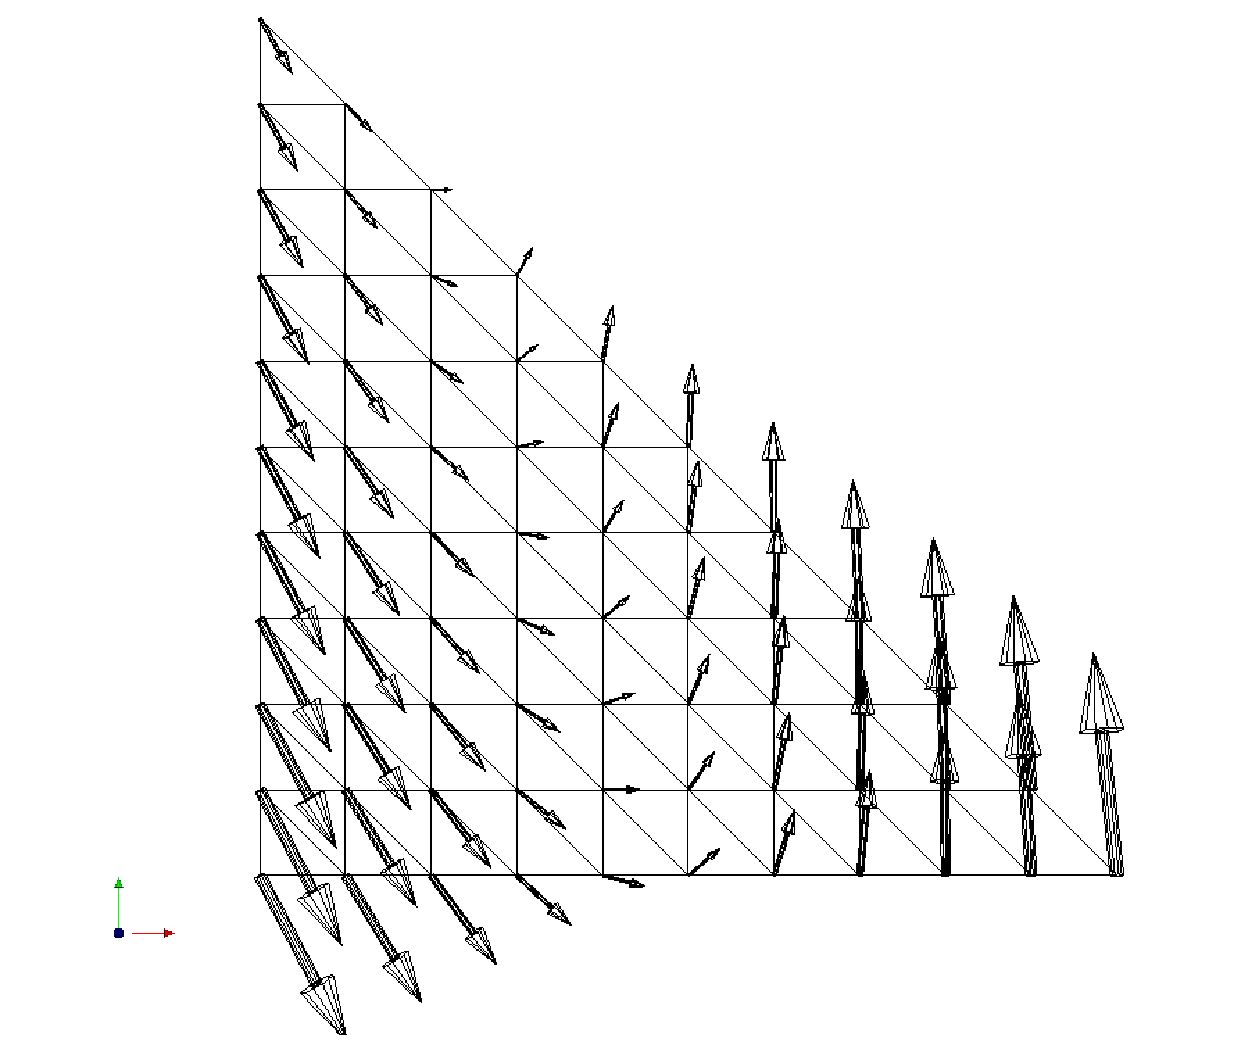
\includegraphics[width=.5\textwidth]{../figures/divfree-2-1-3}
    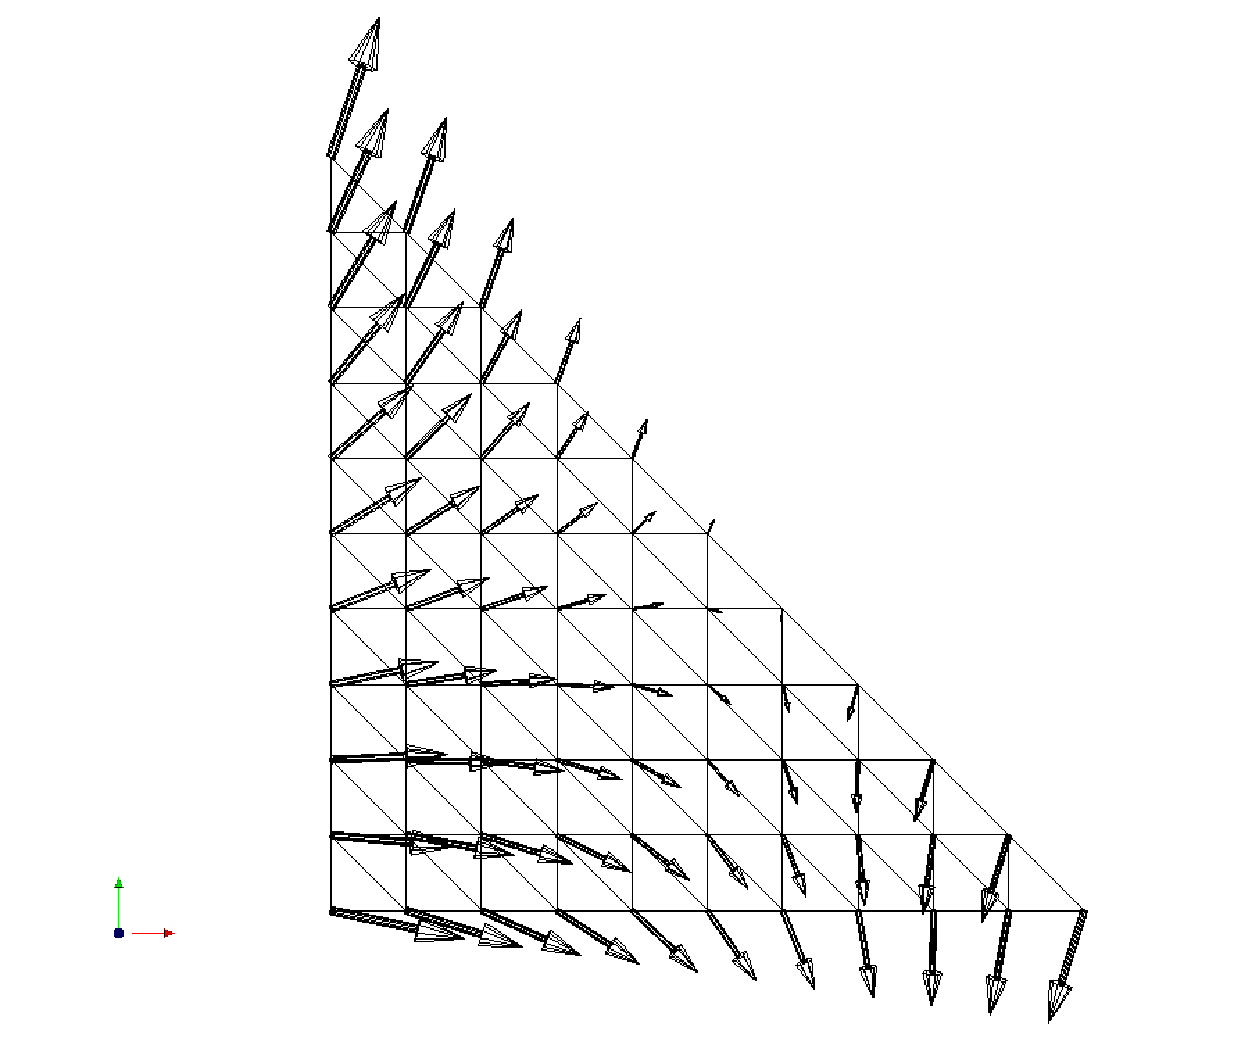
\includegraphics[width=.5\textwidth]{../figures/divfree-2-1-4}
    \caption{2 divergence free polynomials}
    \label{fig:1}
  \end{figure}
\end{frame}

\begin{frame}[label=lag]{$(K,\ \mathbb{P}_k,\ \{\sigma_{x_i}\})$, $(K,\ [\mathbb{P}_k]^d,\ \{\sigma_{x_i}\})$}
  \begin{block}{Lagrange Finite Element}
          \begin{enumerate}
          \item Define $\Pk$
          \item Define $\Sigma=\{\sigma_{x_i}: \Pk \rightarrow \mathbb{R},\ x_i \in K\}$
          \item Order DOFs (continuous/discontinuous)
          \item Given $V$ associated with $\Sigma(\mathbb{P}_k)$,
            solve $V M = I$, $M^T$ contains the coefficients of the
            Lagrange polynomials in the basis of $\Pk$
          \end{enumerate}
      \end{block}
\end{frame}

\begin{frame}[fragile=singleslide]{$(K,\ \mathbb{P}_k,\ \{\sigma_{x_i}\})$, $(K,\ [\mathbb{P}_k]^d,\ \{\sigma_{x_i}\})$}
\begin{lstlisting}[mathescape,basicstyle=\tiny\ttfamily]
template<typename Primal,
         typename ContinuityType, // cG, dG
         class PointSetType>// $\{x_i\}$
class LagrangeDual
 : public DualBasis<Basis>
{
 LagrangeDual( primal_space_type const& primal )
 {
  PointSetType pts; // $\{x_i\}$
  if ( is_continuous )
   { ... } //reorder pts wrt entities

  setFunctionalSet( $\sigma_{\{x_i\}}$( primal, pts ) );
} };
template<uint16_type $d$,
         uint16_type $k$,
         class PolySetType,
         typename ContinuityType = Continuous,
         typename T = double,
         class Convex = Simplex,
         class Pts = PointSetEquiSpaced >
class Lagrange
 : public FiniteElement<
     OrthonormalPolynomialSet<$d$, $k$,
                  PolySetType, T, Convex>,
     LagrangeDual,
     ContinuityType,
     Pts >
{ Lagrange() : FiniteElement<>( dual(primal) ){} };
\end{lstlisting}
\end{frame}

\begin{frame}{$(K,\ \mathbb{P}_k,\ \{\sigma_{x_i}\})$, $(K,\ [\mathbb{P}_k]^d,\ \{\sigma_{x_i}\})$}
  \begin{figure}[H]
    \centering
    \subfigure{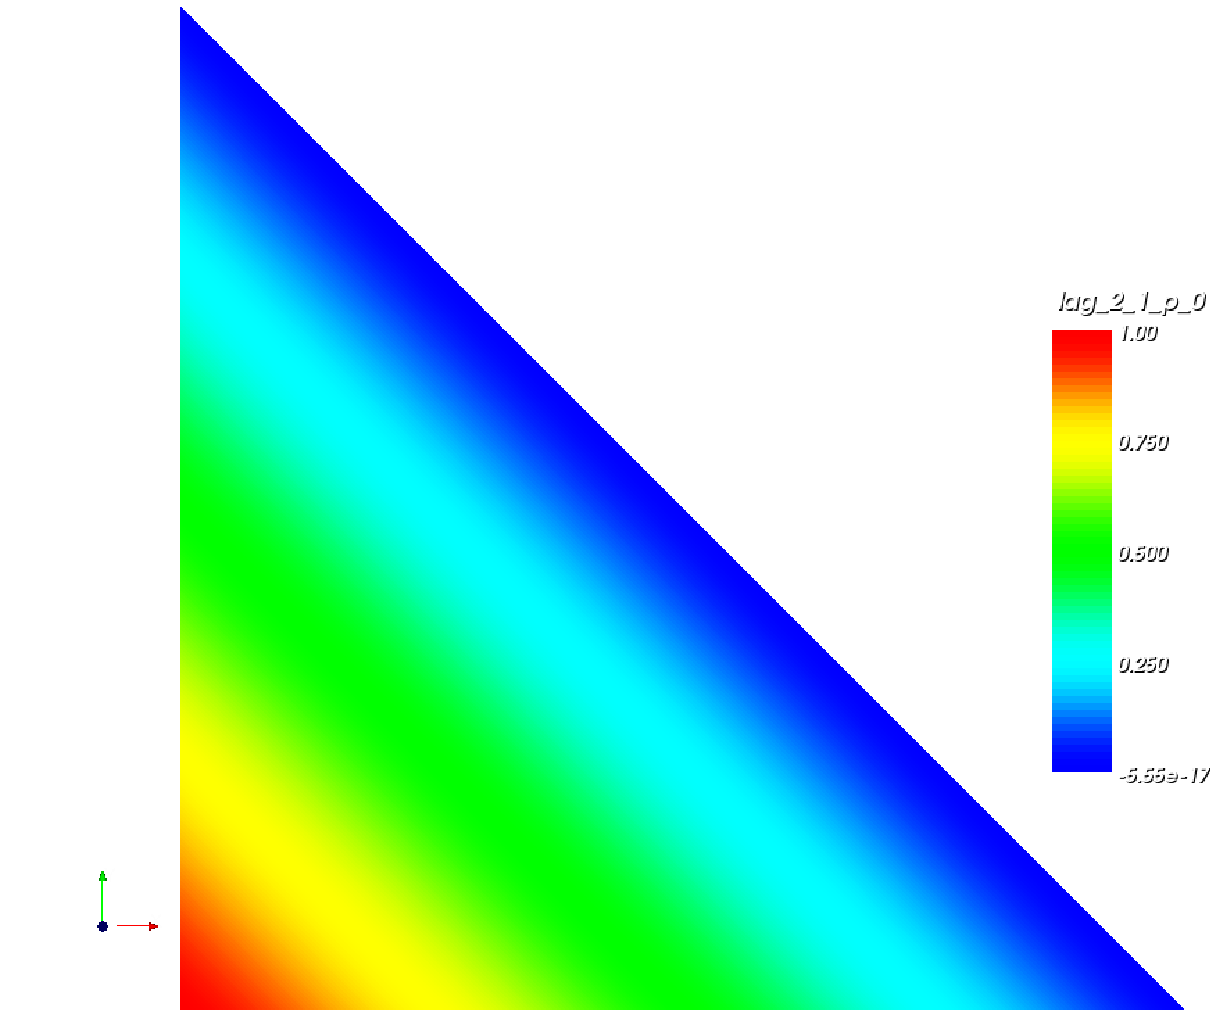
\includegraphics[width=.3\textwidth]{../figures/lag_2_1_p_0.pdf}}
    \subfigure{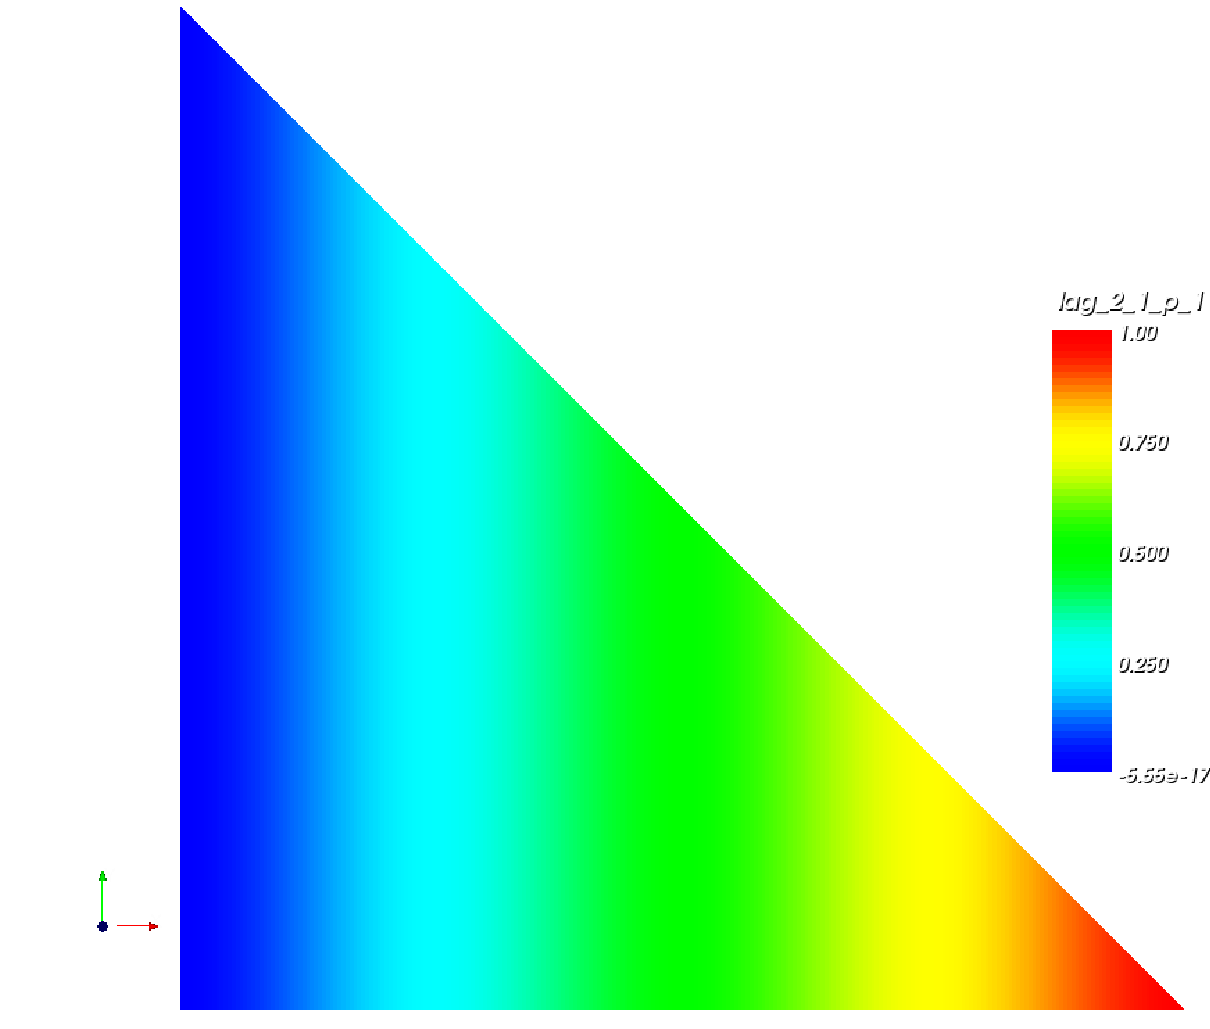
\includegraphics[width=.3\textwidth]{../figures/lag_2_1_p_1.pdf}}
    \subfigure{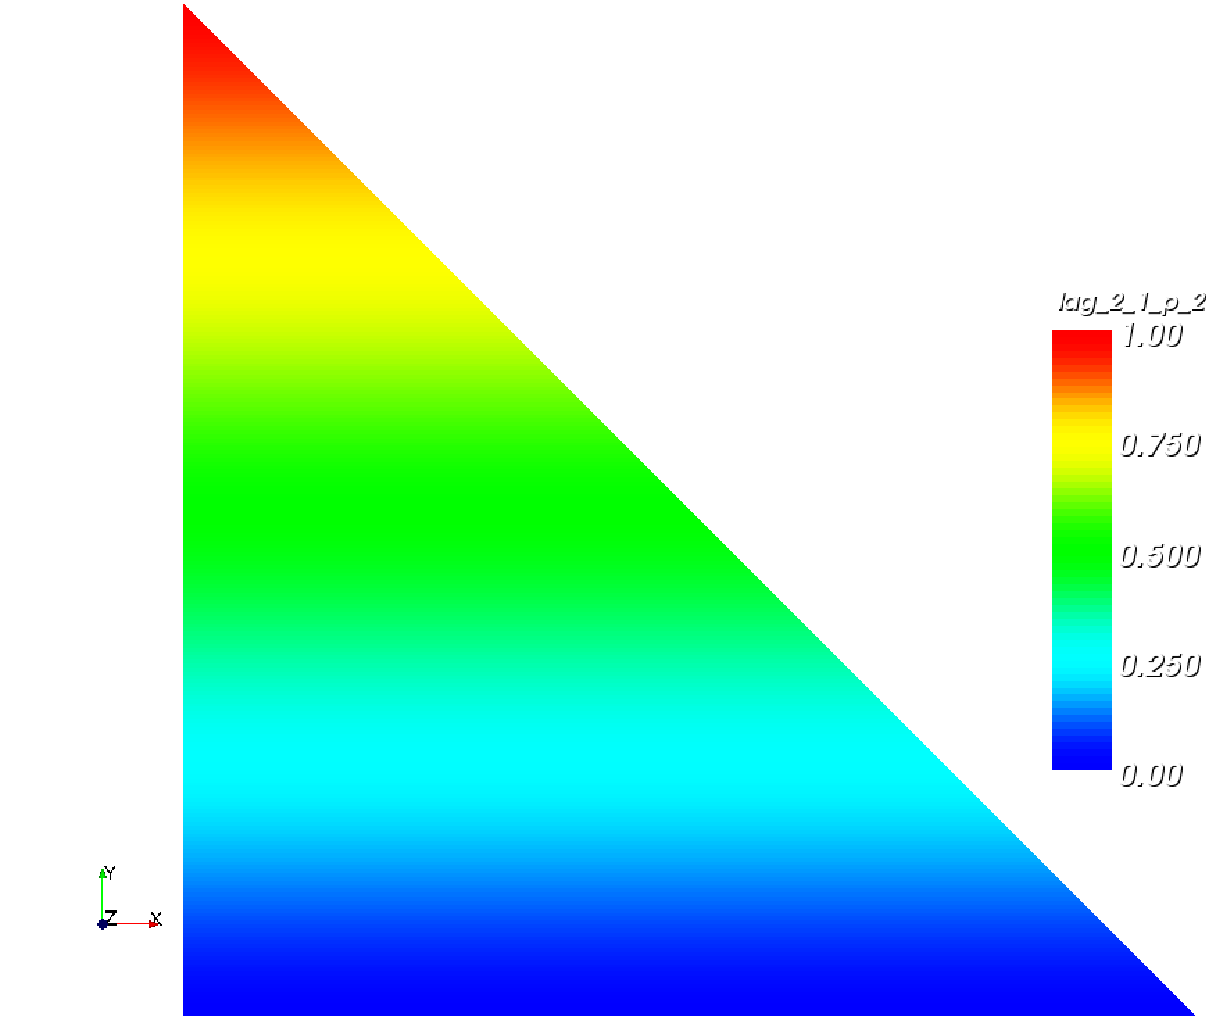
\includegraphics[width=.3\textwidth]{../figures/lag_2_1_p_2.pdf}}\\
    \subfigure{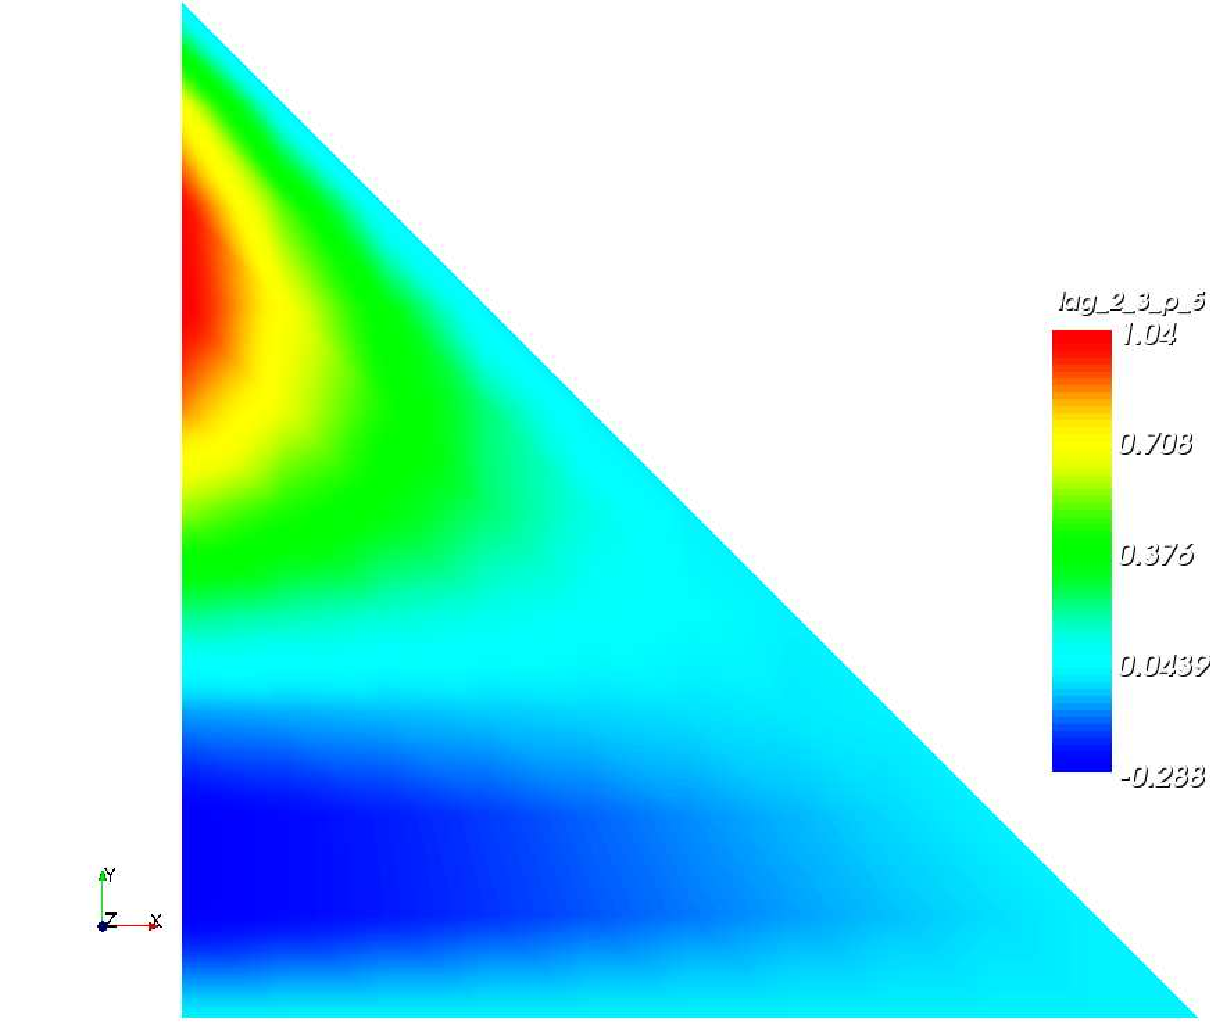
\includegraphics[width=.3\textwidth]{../figures/lag_2_3_p_5.pdf}}
    \subfigure{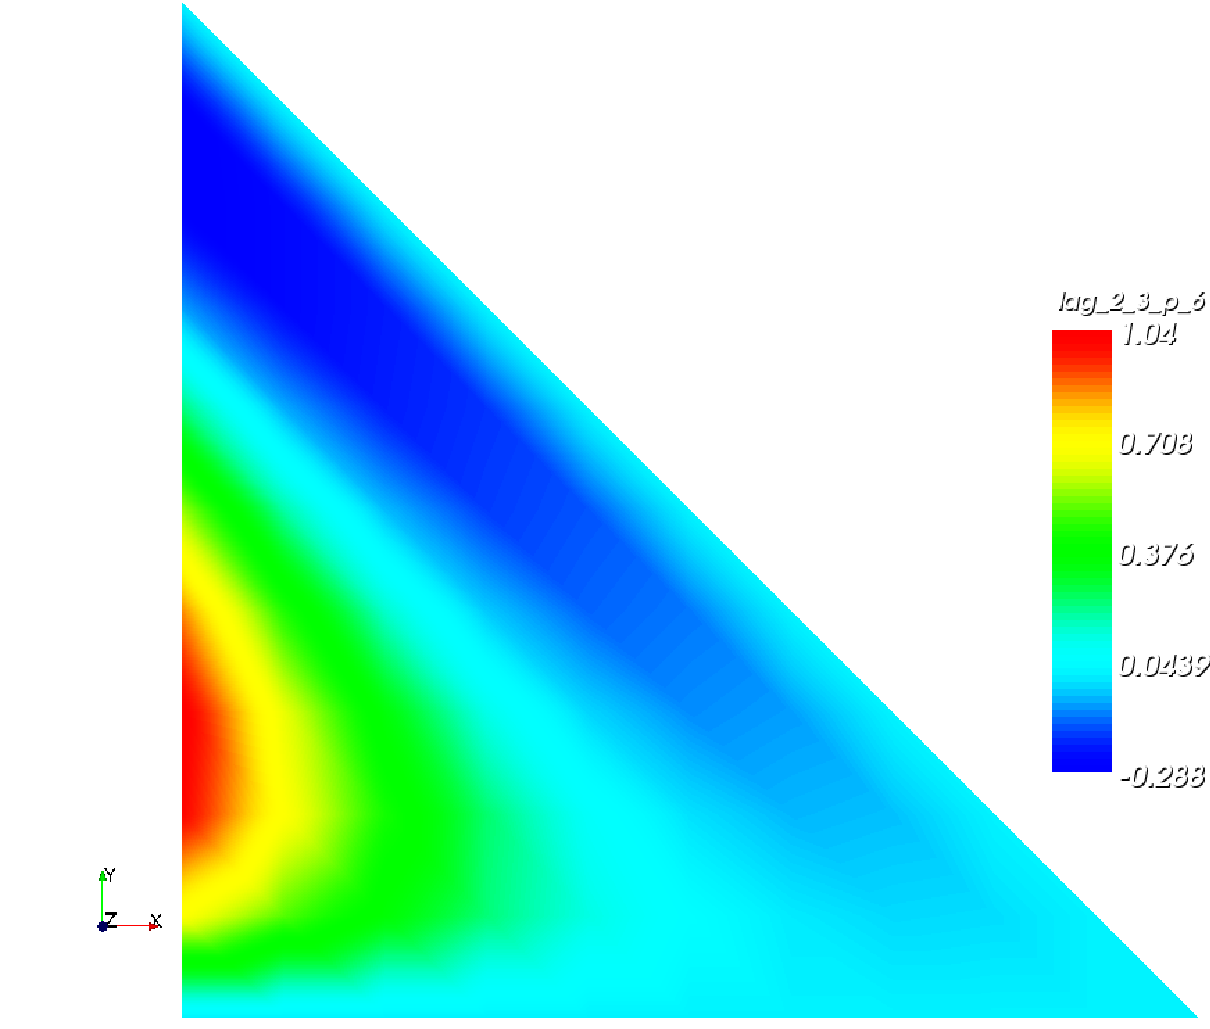
\includegraphics[width=.3\textwidth]{../figures/lag_2_3_p_6.pdf}}
    \subfigure{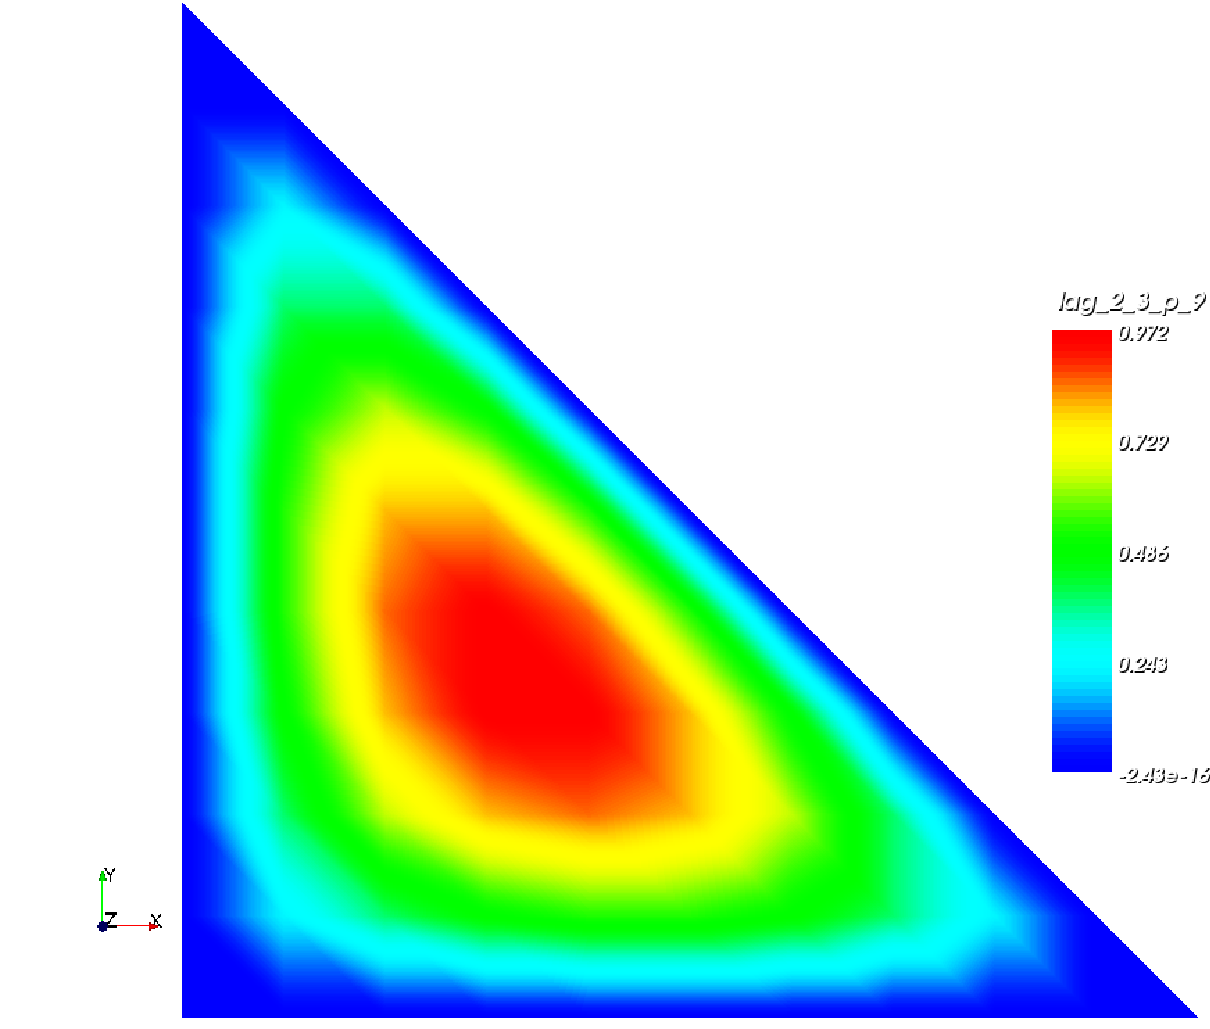
\includegraphics[width=.3\textwidth]{../figures/lag_2_3_p_9.pdf}}
    \caption{Scalar Lagrange element of order 1 (top). Some Lagrange polynomials of degree 3 (bottom)}
  \end{figure}
\end{frame}


\begin{frame}[label=rt]{$(K,\ \mathbb{R}\mathbb{T}_k,\ \{\sigma\})$}
  \begin{block}{Raviart Thomas finite element}
    \begin{enumerate}
    \item Define $$\mathbb{R}\mathbb{T}_k(K) = [\Pk]^d + x \Pk$$
    \item Define the dual space $\Sigma$
    \item Define the set of equidistributed point on the faces $\{x_i, x_i \in \partial K \}$
    \item Define the functional set composed of
      \begin{itemize}
      \item normal component in  $k + 1$ points of each face
      \item moments against a basis of $[\Pkmun]^d$
      \end{itemize}
    \item Apply the functionals of $\Sigma$ to the basis of
      $\mathbb{R}\mathbb{T}_k$, get the matrix $M$
    \item Solve $M V = I$
    \item $V^T$ contains the coefficients of finite element in the
      basis of $\mathbb{R}\mathbb{T}_k$
    \end{enumerate}
  \end{block}
\end{frame}

\begin{frame}[fragile=singleslide]{$(K,\ \mathbb{R}\mathbb{T}_k,\ \{\sigma\})$}
\begin{lstlisting}[mathescape,basicstyle=\tiny\ttfamily]
template<uint16_type $d$,
         uint16_type $k$,
         typename T = double,
         class Convex = $K$>
class RaviartThomasPolynomialSet
 :
  public OrthonormalPolynomialSet<$k$, $k+1$,
                         Vectorial, T, Convex>
{ RaviartThomasPolynomialSet()
  { // $[\mathbb{P}_{k+1}]^d$
    Pkp1_v_type Pkp1_v;
    v_polynomialset_type Pk_v( Pkp1_v.polynomialsUpToDimension( dim_Pk ) );
    // $\mathbb{P}_k$
    Pkp1_s_type Pkp1;
    scalar_polynomialset_type Pk ( Pkp1.polynomialsUpToDimension( dim_Pk ) );
    // $x \mathbb{P}_k\backslash\mathbb{P}_{k-1}$
    IM_PK<convex_type::nDim, 2*nOrder,value_type> im;
    matrix<value_type> xPkc( nComponents*(dim_Pk-dim_Pkm1), Pk.coeff().size2() );
    for( int j = dim_Pkm1, l = 0; j < dim_Pk; ++j, ++l )
    { for( int i = 0; i < convex_type::nDim; ++i )
      {
        times_x<scalar_polynomial_type> xp( Pk.polynomial( j ), i );
        row(xPkc,l*nComponents+i) = row( project( Pkp1,xp, im ).coeff(), 0);
    } }
    v_polynomialset_type xPk( typename super::basis_type(), xPkc );
    // $[\mathbb{P}_k]^d + x \mathbb{P}_k\backslash\mathbb{P}_{k-1}$
    setCoefficient( unite( Pk_v, xPk ).coeff() );  } }
\end{lstlisting}
\end{frame}

\begin{frame}[fragile=singleslide]{$(K,\ \mathbb{R}\mathbb{T}_k,\ \{\sigma\})$}
\begin{lstlisting}[mathescape,basicstyle=\tiny\ttfamily]
template<typename Basis,
    typename ContinuityType,
    template<class, class> class PointSetType>
class RaviartThomasDual
 : public DualBasis<Basis>
{
 // define points on face
 for_each point p in face of convex {
  pts_per_face[p]=convex.makePoints( $d-1$, p ) );
 }
 // compute $ \sigma_f( U ) = (U * n[f]) (p_f)$
 std::vector<functional_type> fset;
 for_each point p in face of convex {
  dcpe_type dcpe( primal, convex.normal(f),
                  pts_per_face[p] );
  std::copy( dcpe.begin(), dcpe.end(),
             std::back_inserter( fset ) ); }
 if ( $k$ > 0 )
 {  Pkp1_v_type Pkp1;
  v_polynomialset_type Pkm1 (
         Pkp1.polynomialsUpToDimension( dim_Pm1 ) );
  for( int i = 0; i < Pkm1.polynomialDimension();
       ++i )
  {
    typedef IntegralMoment<> fim_type;
   fset.push_back( fim_type( primal, Pkm1.polynomial( i ) ) );  }
 }
 setFunctionalSet( fset );}
\end{lstlisting}
\end{frame}

\begin{frame}{$(K,\ \mathbb{R}\mathbb{T}_k,\ \{\sigma\})$}
  \begin{figure}[H]
    \centering
    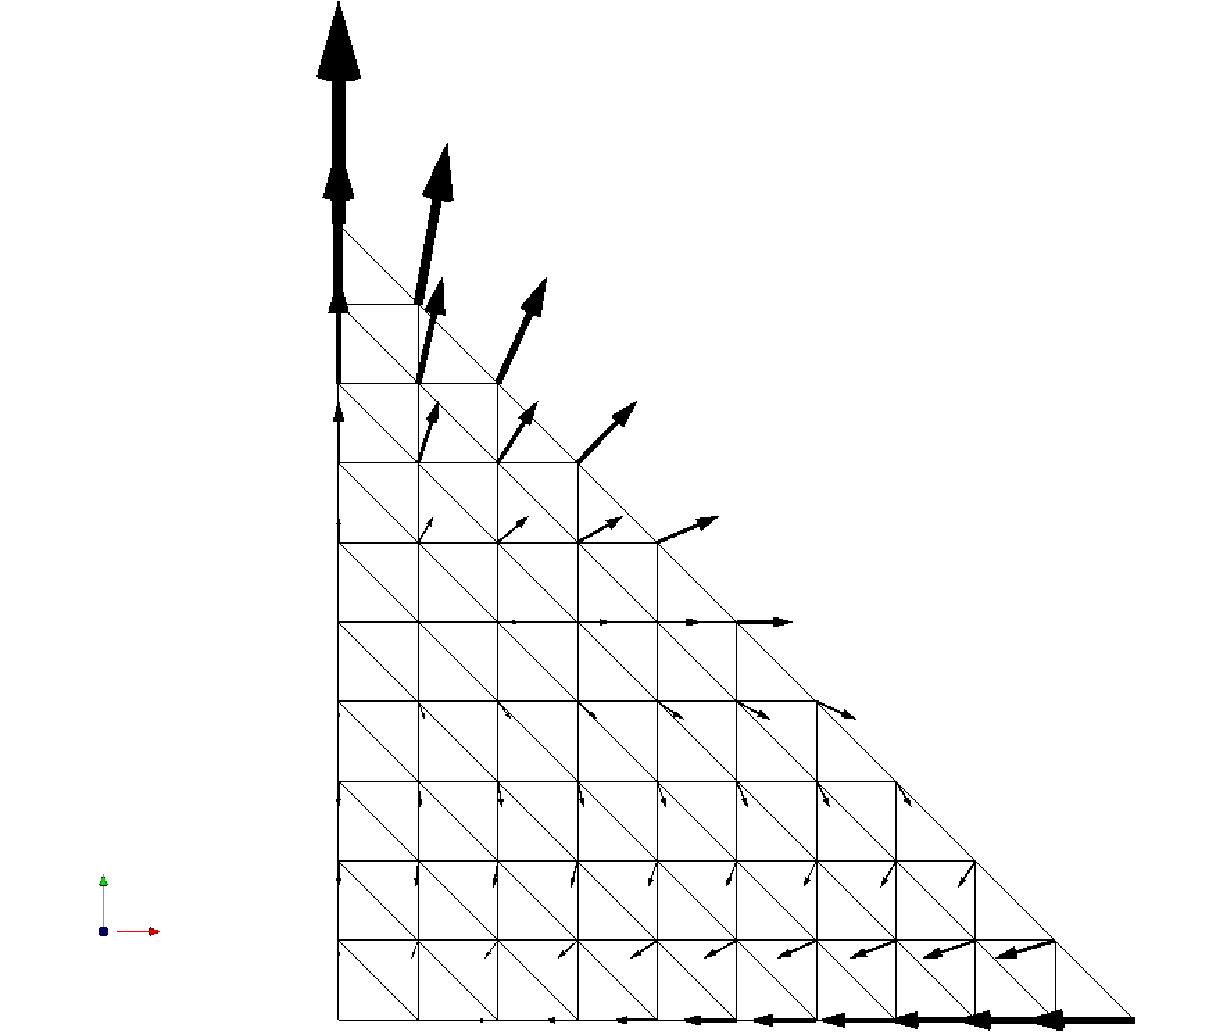
\includegraphics[width=.5\textwidth]{../figures/fert-2-1-1.pdf}
    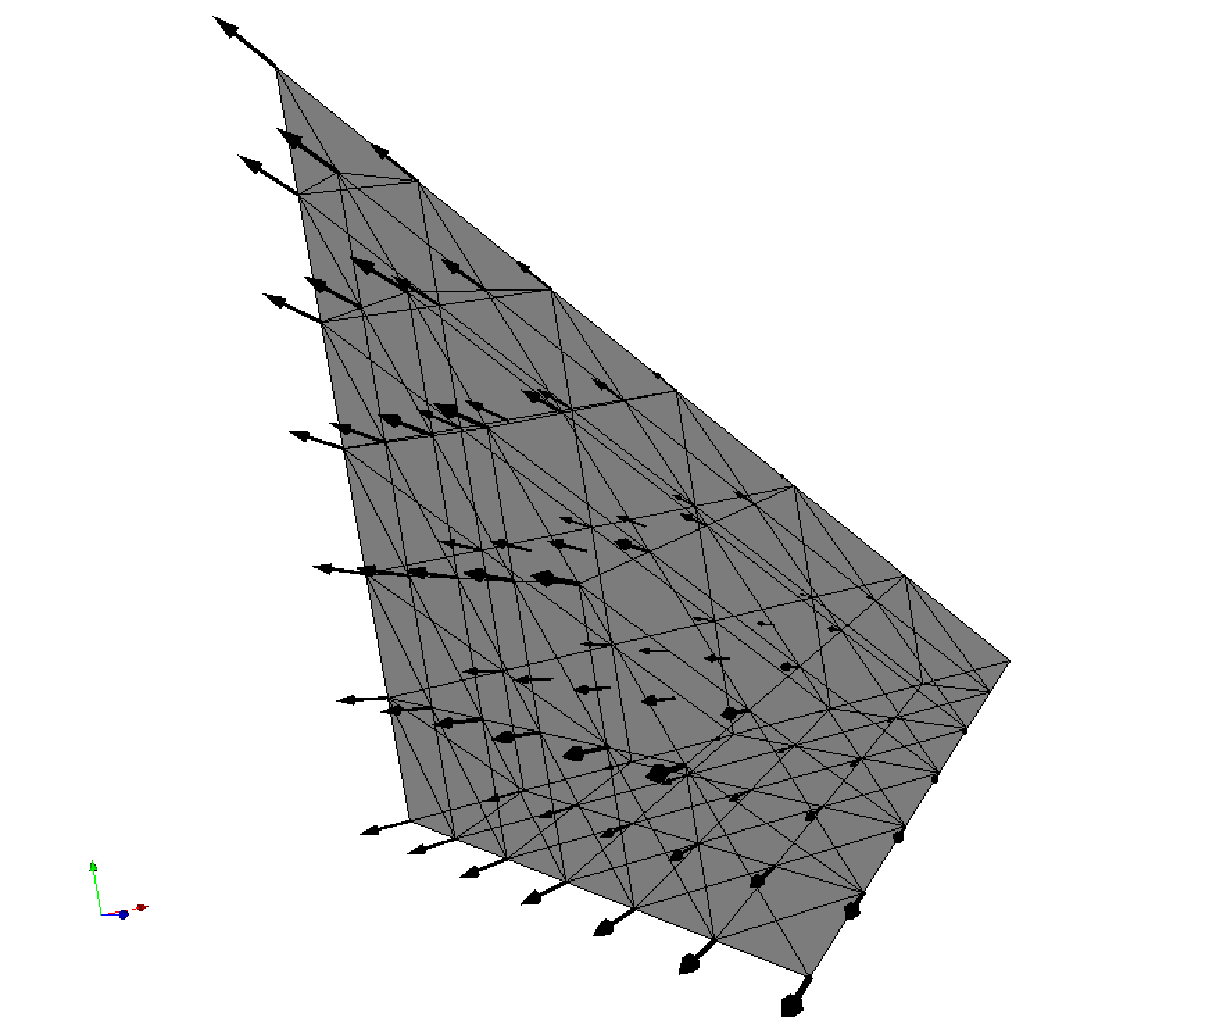
\includegraphics[width=.5\textwidth]{../figures/fert-3-0-1.pdf}
    \caption{2  Raviart-Thomas polynomials in 2D and 3D}
  \end{figure}
\end{frame}


 \subsection{Spectral}


 \begin{frame}{Probl�me 2D sur simplex}
   \begin{columns}
       \begin{column}[c]{.4\textwidth}
 	{\scriptsize
         \begin{figure}[H]
          \centering
 %	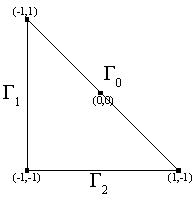
\includegraphics[width=25mm]{../figures/triangle.png}
 	 \movie[externalviewer=kaffeine]{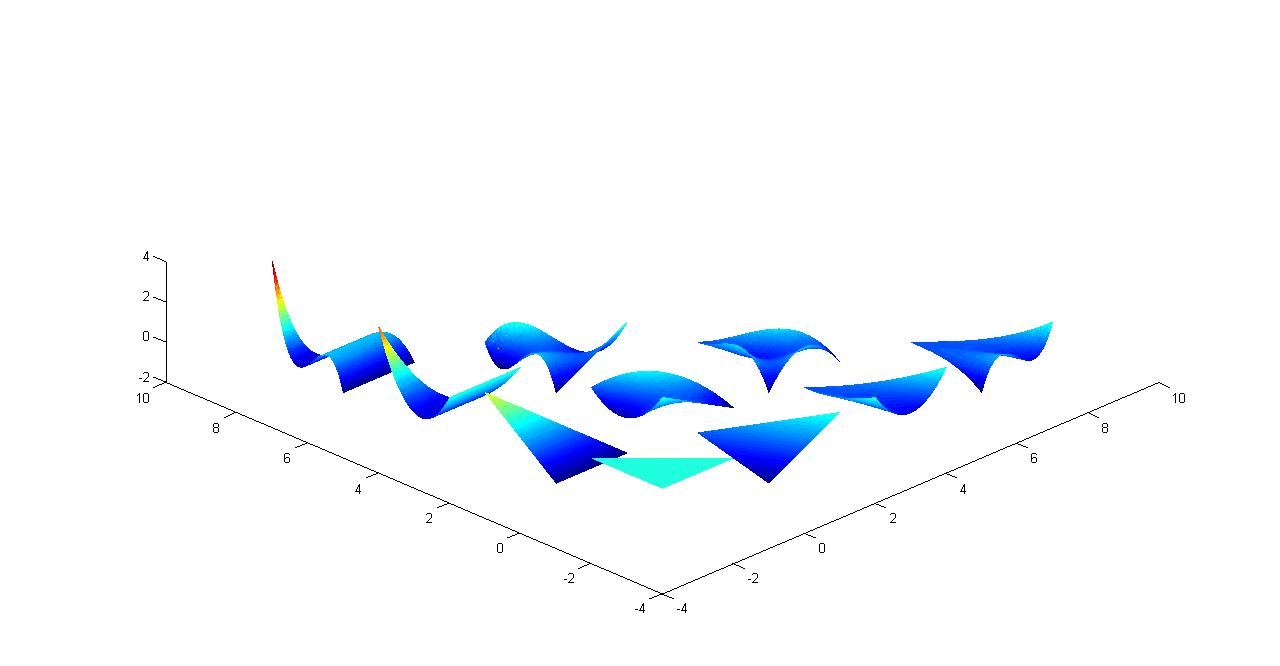
\includegraphics[width=\textwidth]{../figures/Dubiner_3.jpg}}{../figures/Dubiner_5.jpg}
           \caption{\scriptsize Base de Dubiner}
         \end{figure}
 	\begin{itemize}
 	\item Forme forte :
 	$$
 	\left\{
 	\begin{array}{ll}
 	- \Delta u + u = f, & \mbox{ dans } \Omega, \\
 	\frac{\partial u}{\partial \mathbf n_i} = g_i, & \mbox{ sur } \Gamma_i, \\
 	\end{array}
 	\right.
 	$$
 	\item Forme faible :
 	$$
 	\int_{\Omega} \nabla u\nabla v + \int_{\Omega} uv   = \int_{\Omega} fv + \sum_{k=0}^2\int_{\Gamma_k} g_kv
 	$$
 	\end{itemize}
 	}
       \end{column}
       \begin{column}[c]{.6\textwidth}
 	{\scriptsize
 	\begin{itemize}
 	\item Donn�es :
 	\begin{eqnarray*}
 	f &=& (2 \pi^2+1)\sin\pi x \cos\pi y, \\
 	g_0 &=& \pi(\cos \pi x \cos \pi y - \sin \pi x \sin \pi y) / \sqrt{2}, \\
 	g_1 &=& -\pi \cos \pi x \cos \pi y, \\
 	g_2 &=& \pi \sin \pi x \sin \pi y.
 	\end{eqnarray*}
 	\item Solution exacte $\sin \pi x \cos \pi y$ :
  	\begin{figure}[H]
           \centering
           \movie[externalviewer=kaffeine]{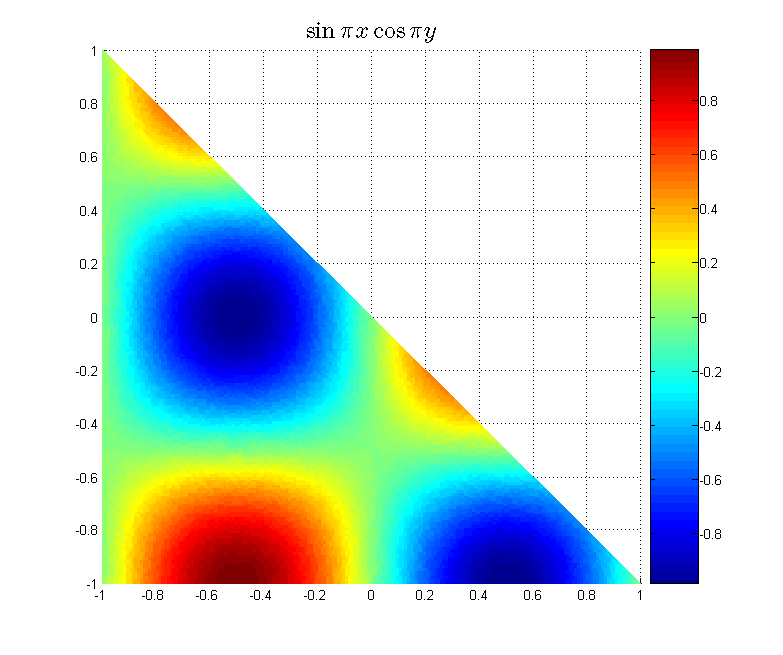
\includegraphics[width=50mm]{../figures/Sol_2D.png}}{../figures/Sol_2D.png}
          \end{figure}
 	\end{itemize}
 	}
       \end{column}
     \end{columns}
\end{frame}
\begin{frame}{Convergence}
     \begin{columns}
      \begin{column}[c]{.5\textwidth}
 	{\scriptsize
 	\begin{itemize}
 	\item Convergence :
         \begin{figure}[H]
          \centering
          \movie[externalviewer=kaffeine]{\hspace{-13mm}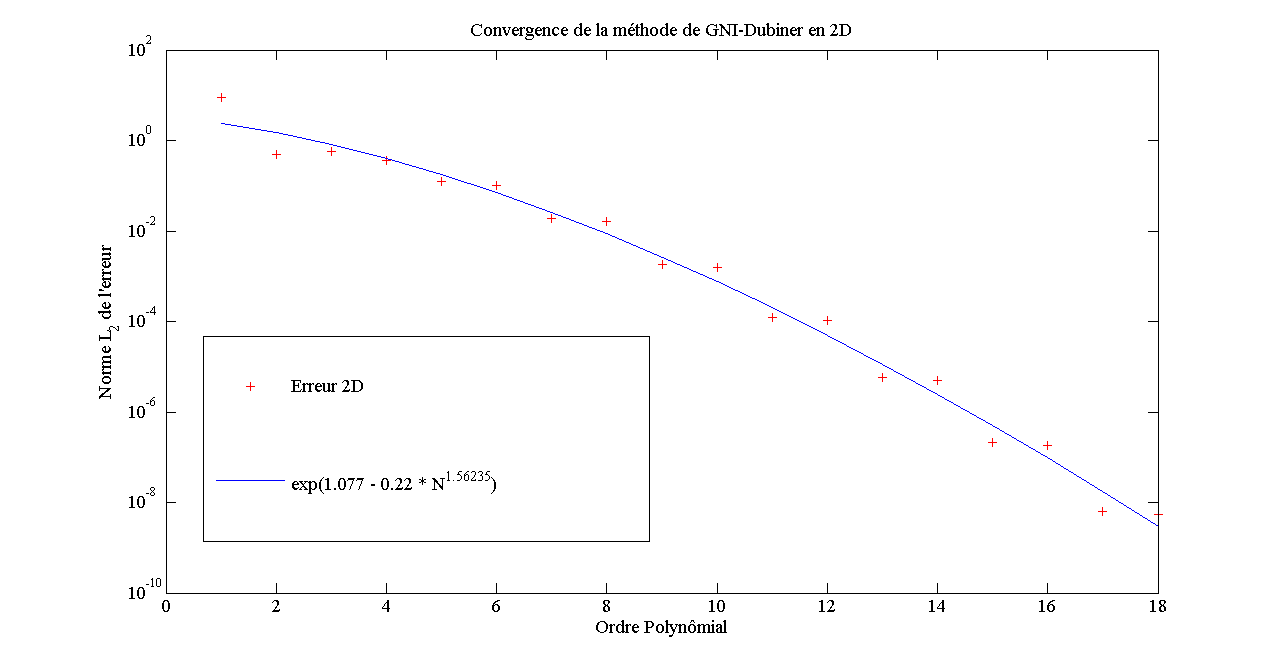
\includegraphics[width=7cm]{../figures/Error_2D.png}}{../figures/Error_2D.png}
         \end{figure}
 	$$
 	\|u - u_N \|_{L^2} \sim  e^{1.077 - 0.22 * N^{1.56235}}
 	$$
 	\end{itemize}
 	}
       \end{column}
       \begin{column}[c]{.5\textwidth}
 	{\scriptsize
 	\vspace{-1mm}
 	\begin{itemize}
 	\item Conditionnement :
 	\begin{figure}[H]
          \centering
          \movie[externalviewer=kaffeine]{\hspace{-10mm}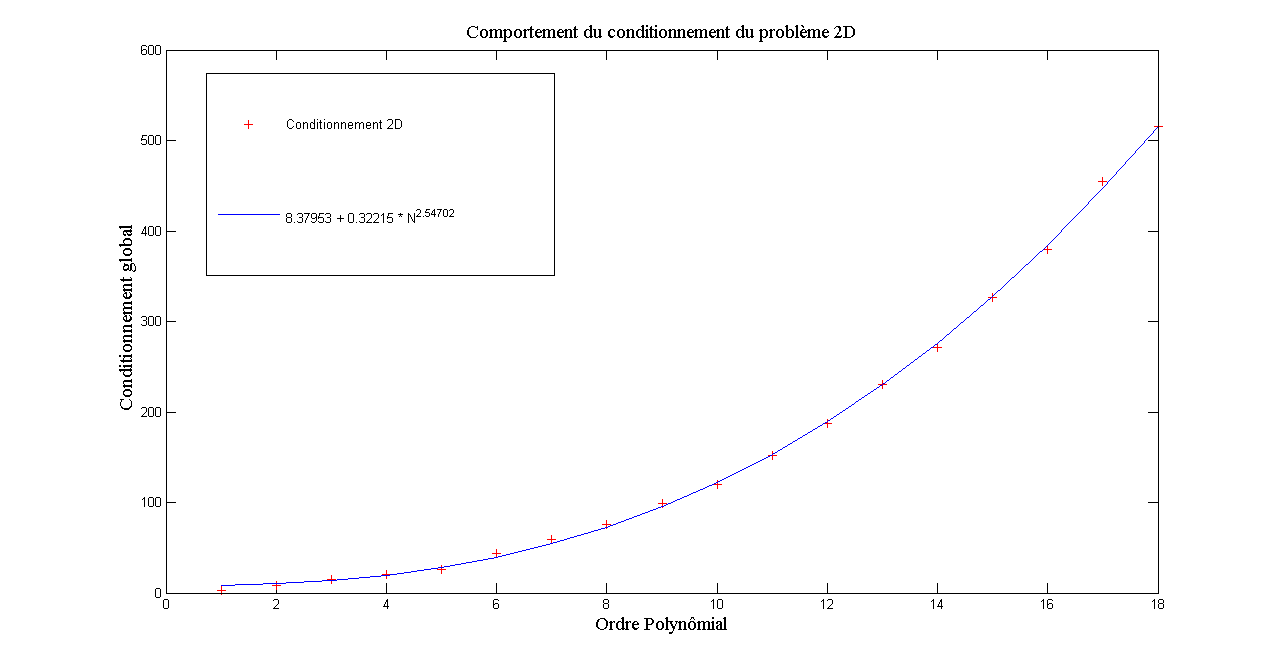
\includegraphics[width=7cm]{../figures/Cond_2D.png}}{../figures/Cond_2D.png}
 	\end{figure}
 	$$
 	\kappa \sim 8.38 + 0.32*N^{2.54702}
 	$$
 	\end{itemize}
 	}
       \end{column}
     \end{columns}
 \end{frame}

 \begin{frame}{Probl�me 3D sur simplex}
     \begin{columns}
       \begin{column}[c]{.4\textwidth}
 	{\scriptsize
         \begin{figure}
          \centering
          %%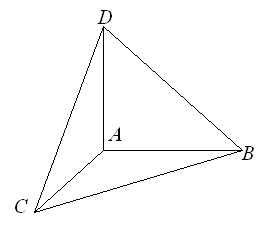
\includegraphics[width=25mm]{../figures/tetra.png}
          \movie[externalviewer=kaffeine]{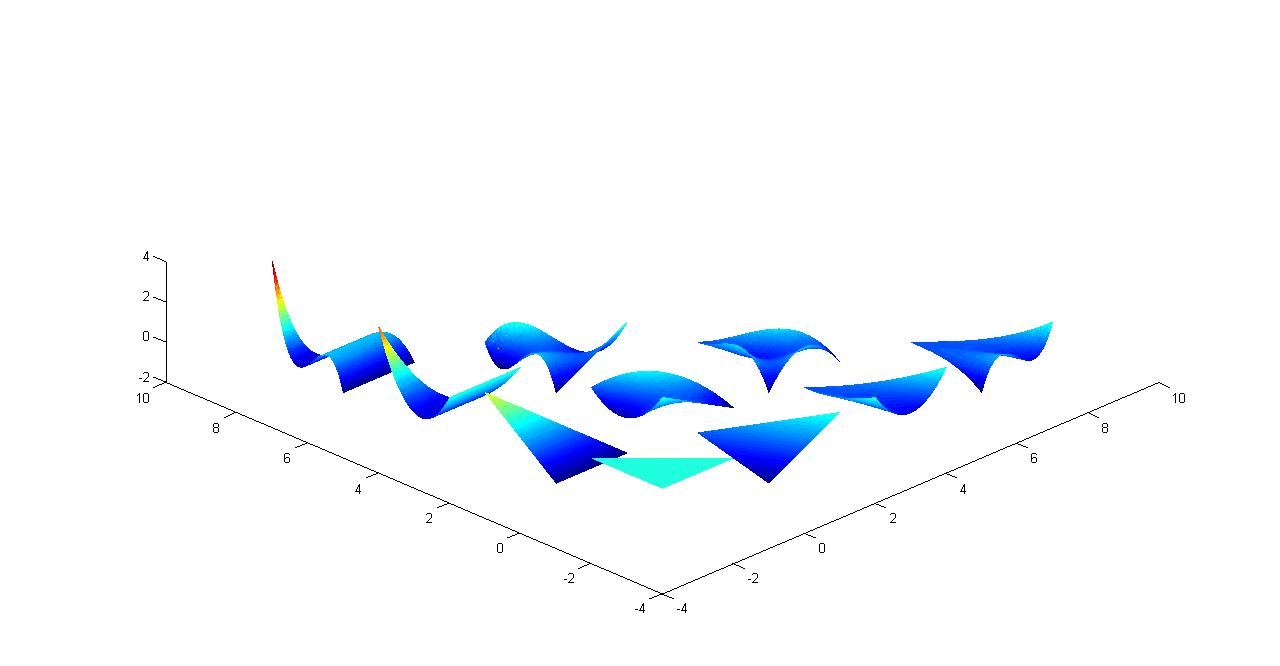
\includegraphics[width=\textwidth]{../figures/Dubiner_3.jpg}}{../figures/Dubiner_5.jpg}
          \caption{\scriptsize Base de Dubiner}
         \end{figure}
 	\begin{itemize}
 	\item Forme forte :
 	$$
 	\left\{
 	\begin{array}{ll}
 	- \Delta u + u = f, & \mbox{ dans } \Omega, \\
 	\frac{\partial u}{\partial \mathbf n_i} = g_i, & \mbox{ sur } \Gamma_i, \\
 	\end{array}
 	\right.
 	$$
 	\item Forme faible :
 	$$
 	\int_{\Omega} \nabla u\nabla v + \int_{\Omega} uv   = \int_{\Omega} fv + \sum_{k=0}^3\int_{\Gamma_k} g_kv
 	$$
 	\end{itemize}
 	}
       \end{column}
       \begin{column}[c]{.6\textwidth}
 	{\scriptsize
 	\begin{itemize}
 	\item Donn�es :
 	\begin{eqnarray*}
 	f &=& (3 \pi^2+1)\sin\pi x \cos\pi y \cos\pi z, \\
 	g_0 &=& \frac{\pi}{\sqrt{3}} (\cos \pi x \cos \pi y \cos\pi z  \\
 	&-& \sin \pi x \sin \pi y \cos\pi z - \sin \pi x \cos \pi y \sin\pi z), \\
 	g_1 &=& -\pi \cos \pi x \cos \pi y \cos\pi z, \\
 	g_2 &=& \pi \sin \pi x \sin \pi y \cos\pi z, \\
 	g_3 &=& \pi \sin \pi x \cos \pi y \sin\pi z.
 	\end{eqnarray*}
 	\item Solution exacte $\sin \pi x \cos \pi y \cos \pi z$.
%  	\begin{figure}[H]
%           \centering
%           \movie[externalviewer=kaffeine]{\includegraphics[width=50mm]{../figures/Sol_3D.png}}{../figures/Sol_3D.png}
%          \end{figure}
 	\end{itemize}
 	}
       \end{column}
     \end{columns}
\end{frame}
\begin{frame}{Convergence}
     \begin{columns}
      \begin{column}[c]{.5\textwidth}
 	{\scriptsize
 	\begin{itemize}
 	\item Convergence :
          \begin{figure}[H]
            \centering
           \movie[externalviewer=kaffeine]{\hspace{-13mm}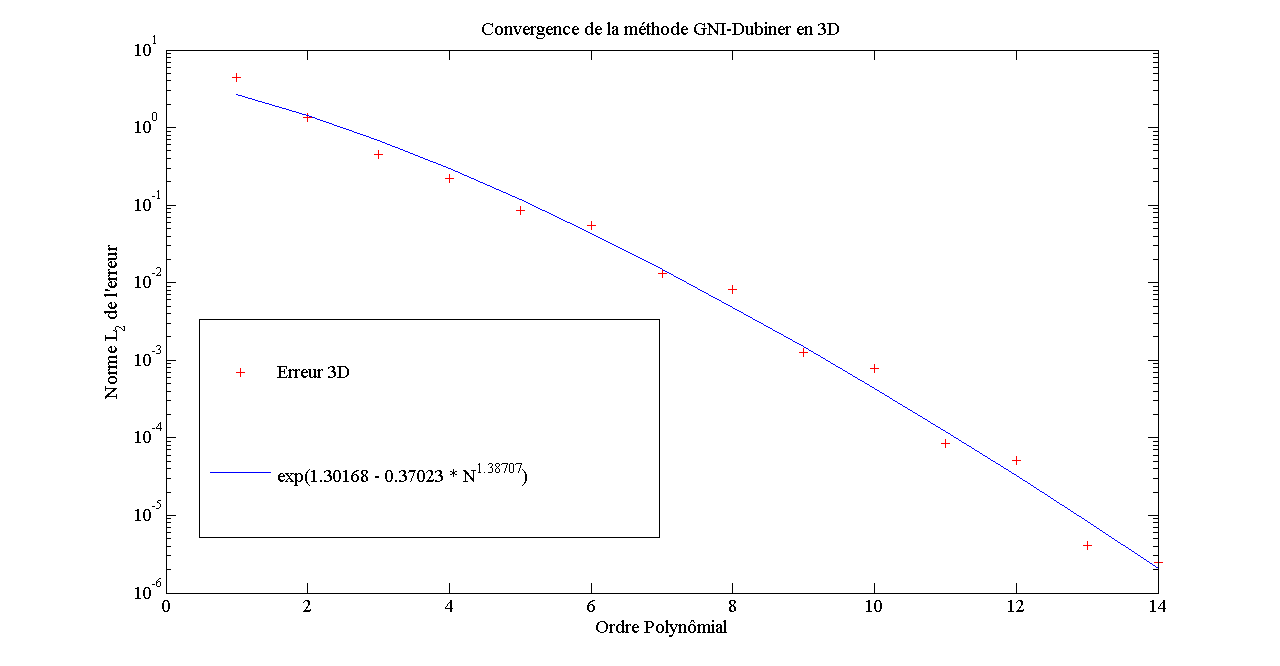
\includegraphics[width=7cm]{../figures/Error_3D.png}}{../figures/Error_3D.png}
         \end{figure}
 	$$
 	\|u - u_N \|_{L^2} \sim  e^{1.30168 - 0.37023 * N^{1.38707}}
 	$$
 	\end{itemize}
 	}
       \end{column}
       \begin{column}[c]{.5\textwidth}
 	{\scriptsize
 	\vspace{-1mm}
 	\begin{itemize}
 	\item Conditionnement :
 	\begin{figure}[H]
          \centering
 	\movie[externalviewer=kaffeine]{\hspace{-10mm}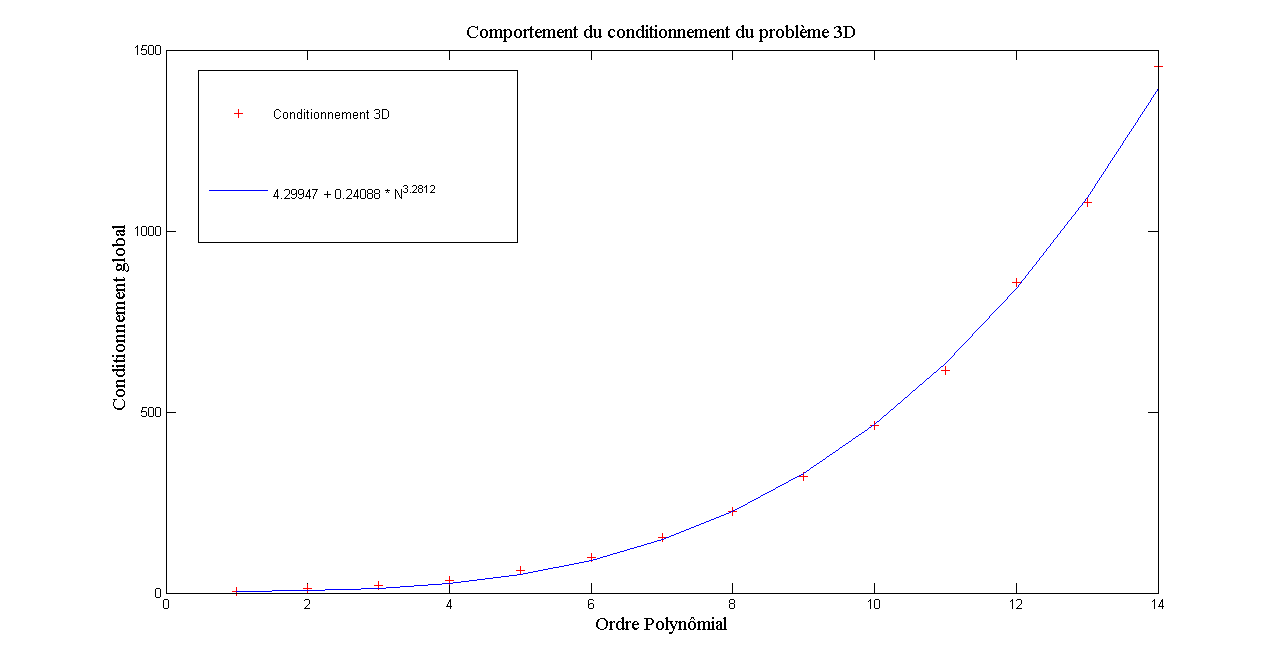
\includegraphics[width=7cm]{../figures/Cond_3D.png}}{../figures/Cond_3D.png}
 	\end{figure}
 	$$
 	\kappa \sim 4.30 + 0.24*N^{3.2812}
 	$$
 	\end{itemize}
 	}
       \end{column}
     \end{columns}
 \end{frame}


\end{document}


\subsection{Newton}
\label{sec:newton}

\begin{frame}{}

\end{frame}

\section[Lagrange]{Lagrange basis}
\label{sec:lagrange-basis}

\subsection{Interpolation}
\label{sec:interpolation}


\begin{frame}{}

\end{frame}

\subsection{Runge Phenomenon}
\label{sec:runge-phenomenon}

\begin{frame}{}

\end{frame}

\subsection{Chebyshev polynomials}
\label{sec:chebysh-polyn}

\begin{frame}{}

\end{frame}

\subsection[Interval]{Interval Approximation}
\label{sec:interv-interp}

\begin{frame}{}

\end{frame}


\section{Multidimension approximation}
\label{sec:mult-interp}

\subsection{Basic geometry}
\label{sec:basic-geometry}

\begin{frame}{}

\end{frame}

\subsection{Coordinate systems}
\label{sec:coordinate-systems}

\begin{frame}{}

\end{frame}

\subsection{Primal basis}
\label{sec:primal-basis}

\begin{frame}{}

\end{frame}

\subsection{Polynomials and set of polynomials}
\label{sec:polyn-set-polyn}

\begin{frame}{}

\end{frame}

\subsection{Functionals and sets of functionals}
\label{sec:functionals}

\begin{frame}{}

\end{frame}

\subsection{Finite elements}
\label{sec:finite-elements}

\begin{frame}{}

\end{frame}

\subsection{Geometric Transformation}
\label{sec:geom-transf}

\begin{frame}{}

\end{frame}

\subsection{Curvilinear domain}
\label{sec:curvilinear-domain}

\begin{frame}{}

\end{frame}


\section{Other Representations}
\label{sec:other-repr}

\subsection{Fourier}
\label{sec:fourier-polynomials}

\begin{frame}{}

\end{frame}


\subsection{Wavelets}
\label{sec:wavelets}

\begin{frame}{}

\end{frame}

\section{MPI}
\label{sec:mpi}

\subsection{Send/Recv}
\label{sec:sendrecv}

\begin{frame}{}

\end{frame}

\section{Programming}
\label{sec:programming}

\subsection{MPI Send/Recv}
\label{sec:mpi-sendrecv}

\begin{frame}{}

\end{frame}

\subsection{C++}
\label{sec:c++}

\begin{frame}{}

\end{frame}

\subsection{Libraries}
\label{sec:libraries}

\begin{frame}{}

\end{frame}



\end{document}


%%% Local Variables:
%%% mode: latex
%%% TeX-master: "scicomp-approx-print"
%%% TeX-PDF-mode: t
%%% TeX-parse-self: t
%%% x-symbol-8bits: nil
%%% TeX-auto-regexp-list: TeX-auto-full-regexp-list
%%% ispell-local-dictionary: "american"
%%% End:

